\section{Livello di trasporto}

\subsection{Introduzione e servizi a livello di trasporto}
Strumento che instaura una \textbf{connessione logica} \textit{end-to-end} tra i processi applicativi dei vari host, \textit{non è un collegamento fisico}.

Il \textbf{livello di trasporto} è in esecuzione sui \textbf{sistemi terminali}, più precisamente nel loro \textit{sistema operativo}, non sui router.
Durante l'invio, al \textit{mittente}, scinde i messaggi in vari \textbf{segmenti}, passandoli al livello inferiore (livello di rete), mentre durante la ricezione, al \textit{destinatario}, riassembla il messaggio.
Il \textbf{livello di trasporto} è un \textbf{daemon}, ovvero un \textit{processo in background} che fornisce servizi, che mette in comunicazione logica i processi, usa i servizi del livello di rete, aspetta dal livello applicativo il messaggio da inviare e a chi inviarlo, fornendo servizi al \textit{livello applicativo}.

Il \textbf{livello di rete} mette in comunicazione logica gli host, quindi una comunicazione \textit{host-to-host}.

\subsubsection{Protocolli utilizzati}
I due protocolli utilizzati sono \textbf{TCP} e \textbf{UDP}.

Il protocollo TCP offre vari servizi, tra cui: controllo di congestione e controllo di flusso, questo garantirà un trasferimento dati \textit{affidabile, ordinato e connection-oriented}, ma avrà ritardi nel trasporto a causa di un maggiore \textit{overhead} e \textit{potenziali ritardi}.

Il protocollo UDP essendo non orientato alla connessione è meno affidabile, non avendo nemmeno i controlli garantiti dal TCP, ma guadagna in velocità, non garantendo il corretto ordine di ricezione dei pacchetti e la ricezione di tutti i pacchetti, offrendo un trasferimento dati \textit{non affidabile, non ordinato e connectionless}, con un \textit{minore overhead} e una \textit{trasmissione più veloce}.

Entrambi i protocolli non garantiscono servizi di \textit{garanzia su ritardi} (visto che non possiamo prevedere il tempo di accodamento, il pacchetto potrebbe perdersi ed essere infinito bloccando tutta la connessione) e \textit{garanzia su ampiezza di banda}, non fornendo garanzie \textit{assolute} su ritardo o ampiezza di banda.

Il passaggio di consegna host-to-host a consegna process-to-process viene chiamato \textbf{multiplexing/demultiplexing a livello di trasporto} (\textit{transport layer multiplexing/demultiplexing}).

\subsection{Multiplexing e demultiplexing}

L'operazione di \textbf{multiplexing} è l'operazione di invio, prende i dati da inviare dai vari processi applicativi, \textit{raccogliendo dati da più processi applicativi}, incapsula il pacchetto con l'intestazione e invia il pacchetto.

L'operazione di \textbf{demultiplexing} è l'operazione di ricezione, prende i vari pacchetti, li ricompatta con le indicazioni dell'intestazione e li manda alla \textbf{socket} (un \textit{endpoint logico} per la comunicazione tra processi, canale di comunicazione virtuale tra \textit{livello applicazione} e \textit{livello di trasporto}) corretta, utilizzando l'intestazione per \textit{consegnare i dati al processo applicativo corretto}.

Nell'intestazione a livello di trasporto abbiamo bisogno di minimo: l'etichetta numerica della socket associata ai processi di mittente e destinatario, quindi il numero porta d'origine e di destinazione. Il resto dei campi, come i numeri di sequenza e i checksum (nel caso di TCP), dipende dal protocollo scelto.

I protocolli \textbf{standard} hanno delle porte precise, motivo per cui già sappiamo qual è la porta di destinazione, usate per \textit{servizi ben noti}.

L'host usa gli indirizzi IP e i numeri di porta per inviare i vari segmenti, identificando \textit{univocamente} un endpoint di comunicazione.

Quindi nel segmento a livello di trasporto avremo il campo con il \textbf{numero di porta di orgine} e il campo col \textbf{numero di porta di destinazione}, i numeri di porta vanno da $0$ a $65535$. Da $0$ a $1023$ abbiamo le \textbf{porte note} (\textit{well-known port number}) e sono riservati per i protocolli applicativi ben noti. 

\subsubsection*{Multiplexing e demultiplexing non orientati alla connessione (UDP)}
Il multiplexing e il demultiplexing UDP funzionano nel seguente modo:
\begin{itemize}
    \item Le socket UDP sono create dalle applicazioni, con il livello di trasporto che assegna automaticamente un numero di porta o con l'applicazione che si lega a una porta specifica.
    \item Il lato client di un'applicazione UDP tipicamente lascia che il livello di trasporto assegni automaticamente il numero di porta, mentre il lato server si lega a una porta specifica.
    \item Durante il multiplexing, il livello di trasporto del mittente crea un segmento UDP che include i dati applicativi, i numeri di porta di origine e destinazione, e altri campi. Il segmento viene poi passato al livello di rete.
    \item Durante il demultiplexing, il livello di trasporto del destinatario esamina il numero di porta di destinazione del segmento UDP e lo consegna alla socket appropriata, e quindi al processo applicativo corretto.
    \item Una socket UDP è identificata univocamente da una coppia composta da indirizzo IP e numero di porta di destinazione. Segmenti con diversi indirizzi IP o numeri di porta di origine, ma con lo stesso indirizzo IP e numero di porta di destinazione, vengono diretti alla stessa socket.
    \item Il numero di porta di origine in un segmento UDP funge da "indirizzo di ritorno". Quando il destinatario vuole inviare una risposta, usa il numero di porta di origine del segmento ricevuto come numero di porta di destinazione del segmento di risposta.
\end{itemize}

\subsubsection*{Multiplexing e demultiplexing orientati alla connessione (TCP)}
Il demultiplexing TCP si basa sull'identificazione delle socket TCP tramite una quaterna: indirizzo IP di origine, numero di porta di origine, indirizzo IP di destinazione e numero di porta di destinazione. Questa quaterna identifica univocamente una connessione TCP. A differenza di UDP, segmenti TCP con indirizzi IP o numeri di porta di origine diversi vengono diretti a socket differenti, anche se l'indirizzo IP e la porta di destinazione sono uguali (eccetto per i segmenti di richiesta di connessione).
\begin{itemize}
    \item Un server TCP ha una "socket di benvenuto" in ascolto su una porta specifica, usata per accettare nuove connessioni.
    \item Un client TCP crea una socket e invia un segmento con il flag SYN impostato a 1 per stabilire la connessione. Il sistema operativo del client sceglie un numero di porta di origine.
    \item Il server, ricevuta la richiesta di connessione, crea una nuova socket di connessione e memorizza la quaterna.
    \item Tutti i segmenti successivi con la stessa quaterna vengono diretti alla socket di connessione corrispondente.
    \item Un server può gestire più connessioni TCP concorrenti, ognuna identificata da una quaterna univoca.
\end{itemize}
Anche se più client usano la stessa porta di origine, il server può distinguere le connessioni grazie ai diversi indirizzi IP di origine.

\subsection{Trasporto senza connessione: UDP}
Un protocollo senza connessione, ciò significa che UDP non stabilisce una connessione prima di inviare i dati, i segmenti (NON SONO DATAGRAMMI) UDP (User Datagram Protocol) possono essere perduti o consegnati in ordine errato. UDP non garantisce la consegna, l'ordine o l'assenza di duplicati.

L'intestazione UDP è formata da numero porta origine, numero porta di destinazione, lunghezza in byte del segmento UDP con intestazione e il checksum (che è \textit{opzionale} in IPv4, aggiunge bit alla fine per controllare se viene corrotto il pacchetto), tutti tasselli da 16 bit, totale di 8 Byte.

\begin{center}
  \begin{tabular}{|c|c|c|}
    \hline
    \multicolumn{2}{|c|}{\textbf{Source Port Number}} & \multicolumn{1}{c|}{\textbf{Destination Port Number}} \\
    \multicolumn{2}{|c|}{(2 bytes - 16 bit)} & \multicolumn{1}{c|}{(2 bytes - 16 bit)} \\ \hline
    \multicolumn{2}{|c|}{\textbf{Length}} & \multicolumn{1}{c|}{\textbf{Checksum}} \\
    \multicolumn{2}{|c|}{(2 bytes - 16 bit)} & \multicolumn{1}{c|}{(2 bytes - 16 bit)} \\ \hline
    \multicolumn{3}{|c|}{\textbf{Payload Data (If Any)}} \\
    \multicolumn{3}{|c|}{(variable length)} \\ \hline
  \end{tabular}
\hspace{0.5cm}
\end{center}

UDP viene usato nei protocolli \textbf{DNS} e \textbf{SNMP}, viene utilizzato nelle applicazioni multimediali, che sono \textit{sensibili alla latenza} e tollerano la perdita di dati.

\subsubsection*{Checksum UDP}

Serve a rilevare gli \textit{errori di bit} nel segmento trasmesso, controlla se ci sono bit alternati nella checksum confrontandolo con il checksum prima del trasporto.

Operazioni del mittente:
\begin{itemize}
  \item Somma tutte le parole (tutti i campi presenti nel campo UDP, compreso di intestazione) tradotte in binari, usando l'\textit{aritmetica del complemento a uno}. Nel caso in cui ci sia un riporto (17 bit) lo sommo al bit meno significativo, quindi il primo bit viene sommato al diciasettesimo bit, questa operazione è chiamata \textit{end-around carry}, così che ora il pacchetto è lungo 16 bit.
  \item La checksum è il complemento a 1 della somma (gli 1 diventano 0 e gli 0 diventano 1).
  \item Il client calcola il checksum sull'\textit{intero segmento UDP}, inclusi header e dati, e lo mette nell'intestazione.
\end{itemize}

L'host calcola il checksum e lo controlla con quello dentro l'intestazione, se rileva una discrepanza, ovvero se il checksum \textit{ricalcolato} non corrisponde a quello ricevuto, scarta il pacchetto.

Errori multipli possono annullare bit corrotti, essendo somma binaria, se due bit opposti si corrompono il risultato non cambia. Il checksum non è quindi \textit{infallibile} e può non rilevare alcuni errori.

\subsection{Principi del trasferimento dati affidabile}
Il servizio che offre il livello di trasporto è di un \textbf{canale affidabile}, ma l'implementazione del servizio utilizza un \textbf{canale inaffidabile} realizzato dal \textbf{livello di rete}. Il livello di trasporto deve realizzare il collegamento e rendere affidabile il canale messo a disposizione dal livello di rete.

\begin{center}
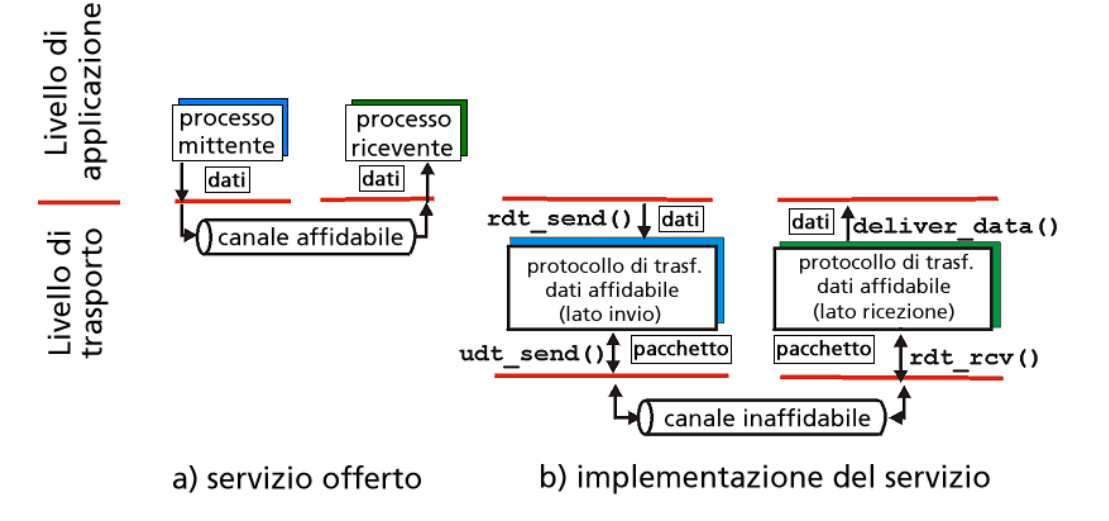
\includegraphics[width=\textwidth]{./img/implemntazionelivellotrasporto.png} 
\textit{rdt: reliable data transfer} - \textit{udt: unreliable data transfer}
\end{center}

Il livello di trasporto, quindi, implementa un protocollo di trasferimento dati affidabile (rdt) per fornire un canale affidabile al livello applicativo, nonostante l'inaffidabilità del livello di rete. Il protocollo rdt utilizza funzioni come \texttt{rdt\_send()} per inviare dati e \texttt{deliver\_data()} per consegnare i dati al livello applicativo. Per comunicare attraverso il canale inaffidabile, il protocollo rdt utilizza funzioni come \texttt{udt\_send()} per inviare pacchetti e \texttt{rdt\_rcv()} per riceverli.

\subsubsection*{Rdt1.0: Mondo ideale}
In un mondo ideale dove il livello rete offre un \textbf{canale affidabile}, il livello di trasporto esegue solo queste operazioni:
\begin{itemize}
  \item L'host riceve i dati da inviare e il destinatario dal livello applicativo.
  \item Crea i pacchetti da inviare.
  \item Invia i dati al destinatario tramite il livello di rete.
  \item \dots
  \item Il client riceve i dati dal livello di rete.
  \item Estrae i dati.
  \item Invia i dati al livello applicativo.
\end{itemize}

\begin{center}
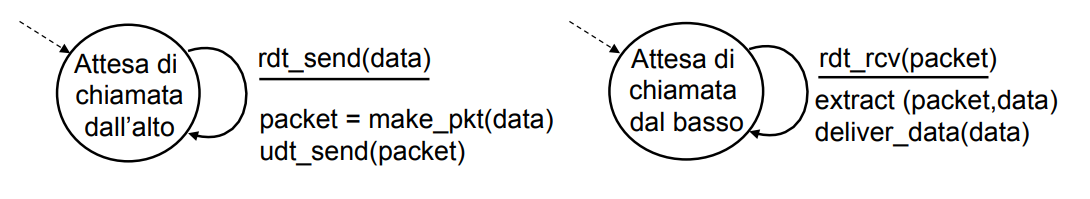
\includegraphics[width=\textwidth]{./img/rdt1.0.png}
\end{center}

Il protocollo \texttt{rdt1.0} rappresenta un caso ideale in cui il livello di rete fornisce un canale di comunicazione perfetto. Il mittente, in attesa di una chiamata dal livello applicativo, invia i dati ricevuti tramite la funzione \texttt{rdt\_send(data)}, creando un pacchetto con \texttt{make\_pkt(data)} e inviandolo con \texttt{udt\_send(packet)}. Il destinatario, in attesa di una chiamata dal livello di rete, riceve il pacchetto con \texttt{rdt\_rcv(packet)}, estrae i dati con \texttt{extract(packet,data)} e li consegna al livello applicativo con \texttt{deliver\_data(data)}.

\subsubsection*{Rdt2.0: canale con errori nei bit}
Il \textit{livello di trasporto} riceve i dati dal \textit{livello applicativo}, crea i pacchetti e aggiunge all'intestazione la checksum a ogni pacchetto.
Invia il pacchetto al destinatario che ricalcolerà il checksum e controllerà se è corretto. Nel caso in cui sia corretto, manderà un messaggio di \textbf{ACK} (conferma di ricezione) al mittente e manderà il pacchetto al \textit{livello applicativo} del destinatario. Altrimenti, manderà un messaggio di \textbf{NAK} (notifica pacchetto corrotto) al mittente che dovrà rimandare lo stesso pacchetto prima di procedere a inviare i restanti.

\begin{center}
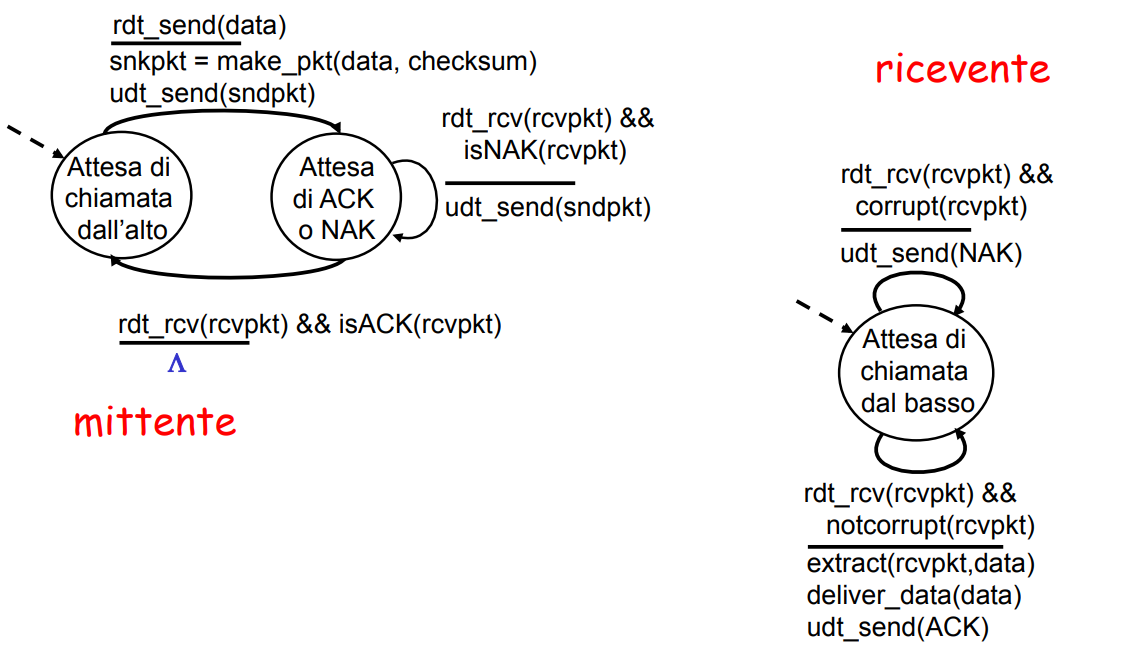
\includegraphics[width=\textwidth]{./img/rdt2.0.png}
\end{center}

Il protocollo \texttt{rdt2.0} introduce la gestione degli errori di bit. Il mittente, in attesa di una chiamata dal livello applicativo, crea un pacchetto con checksum tramite \texttt{make\_pkt(data, checksum)} e lo invia con \texttt{udt\_send(sndpkt)}. Il mittente poi attende un ACK o un NAK. Se riceve un NAK o un pacchetto corrotto (tramite \texttt{rdt\_rcv(rcvpkt) \&\& isNAK(rcvpkt)}), ritrasmette il pacchetto. Se riceve un ACK (tramite \texttt{rdt\_rcv(rcvpkt) \&\& isACK(rcvpkt)}), torna allo stato di attesa. Il destinatario, in attesa di una chiamata dal livello di rete, riceve un pacchetto con \texttt{rdt\_rcv(rcvpkt)}. Se il pacchetto è corrotto (tramite \texttt{corrupt(rcvpkt)}), invia un NAK con \texttt{udt\_send(NAK)}. Se il pacchetto non è corrotto (tramite \texttt{rdt\_rcv(rcvpkt) \&\& notcorrupt(rcvpkt)}), estrae i dati con \texttt{extract(rcvpkt,data)}, li consegna al livello applicativo con \texttt{deliver\_data(data)} e invia un ACK con \texttt{udt\_send(ACK)}.

\subsubsection*{Rdt2.1: il mittente gestisce gli ACK o NAK alterati}
Un problema di questo metodo è il caso in cui i pacchetti di \textit{ACK} o \textit{NAK} vengano corrotti, quindi il mittente non sa la risposta corretta del destinatario. Ritrasmettere è un'opzione, ma si possono avere dei \textbf{duplicati}.
Dobbiamo risolvere il problema dei \textit{duplicati}, aggiungiamo il \textbf{numero di sequenza} a ogni pacchetto. Il ricevente scarterà il pacchetto duplicato nel caso in cui il mittente rimandi lo stesso pacchetto anche avendo già mandato un \textit{ACK}, avendo già memorizzato il \textit{numero di sequenza}.

Schema automa a stati finiti mittente:
\begin{center}
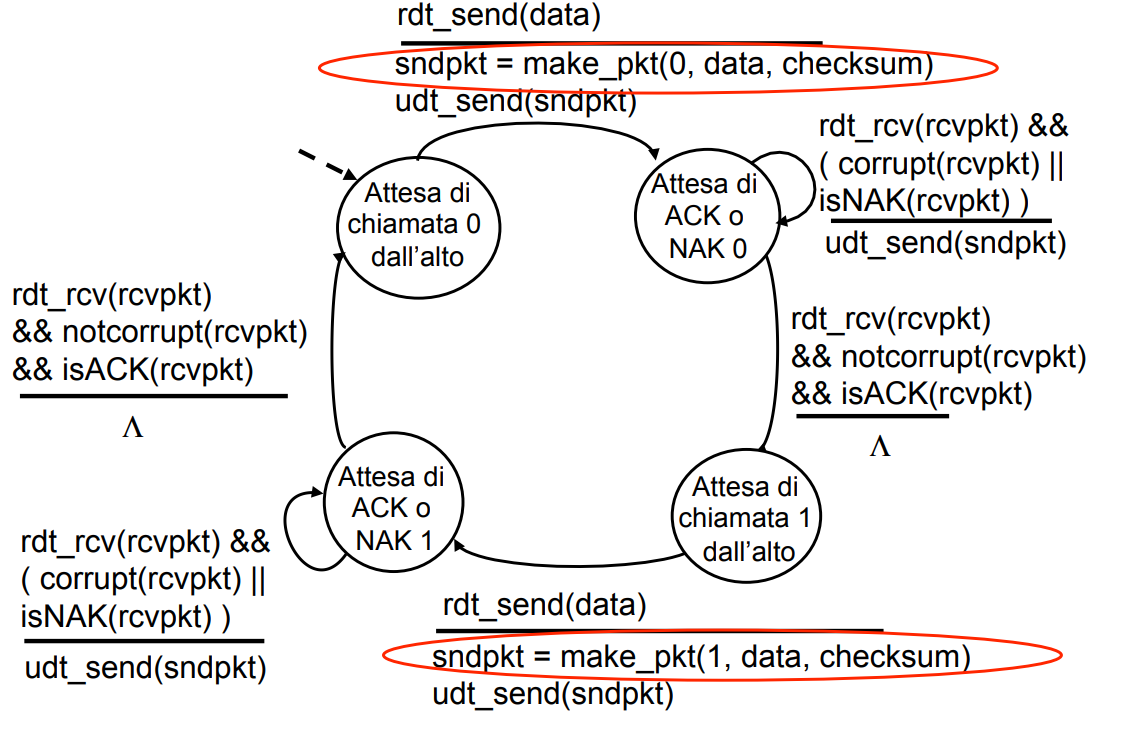
\includegraphics[width=\textwidth]{./img/rdt2.1mit.png}
\end{center}

Schema automa a stati finiti ricevente:
\begin{center}
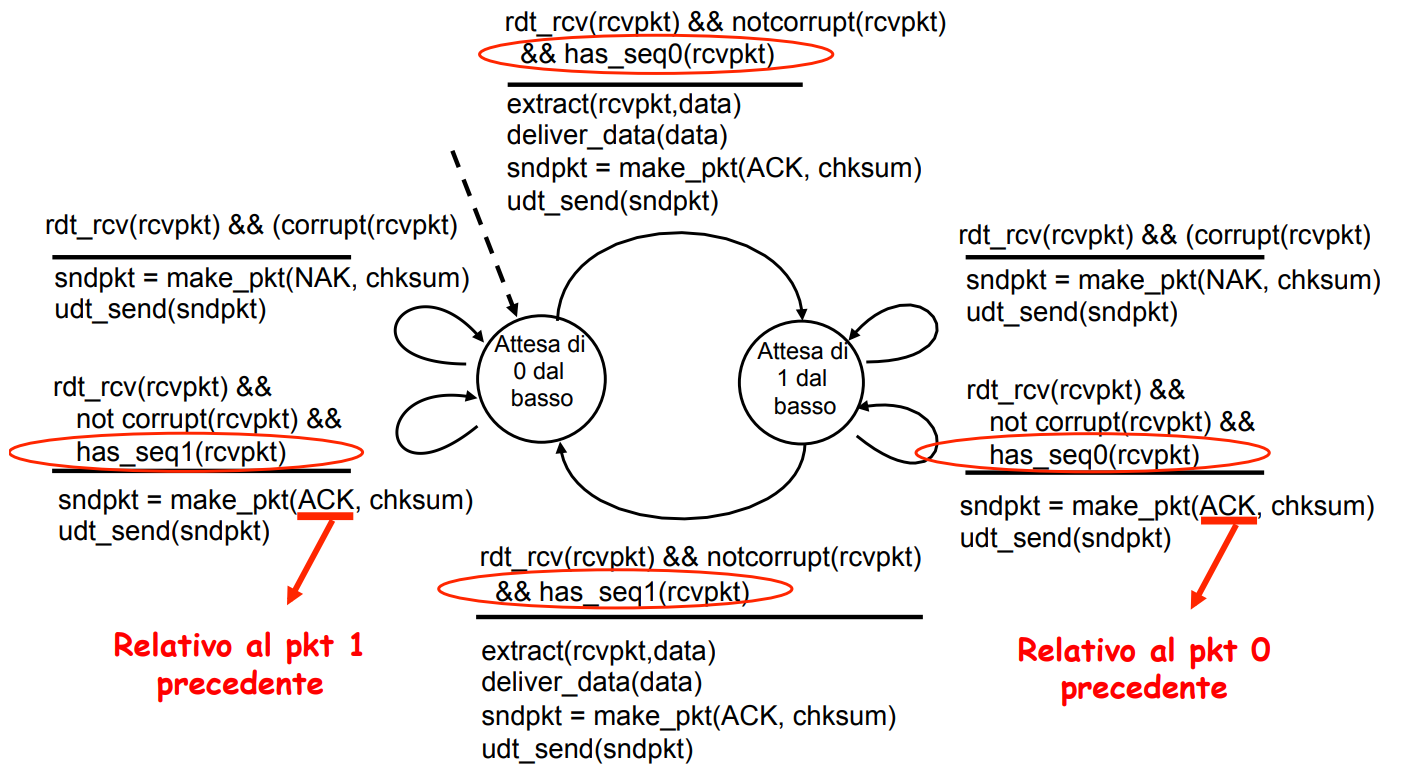
\includegraphics[width=\textwidth]{./img/rdt2.1ric.png}
\end{center}

Il protocollo \texttt{rdt2.1} introduce i numeri di sequenza per gestire i duplicati. Il mittente, in attesa di una chiamata dal livello applicativo, crea un pacchetto con numero di sequenza (0 o 1) e checksum tramite \texttt{make\_pkt(seq, data, checksum)} e lo invia con \texttt{udt\_send(sndpkt)}. Il mittente poi attende un ACK o un NAK.

Se riceve un NAK o un pacchetto corrotto (tramite \texttt{rdt\_rcv(rcvpkt) \&\& (corrupt(rcvpkt) || isNAK(rcvpkt))}), ritrasmette il pacchetto. Se riceve un ACK non corrotto (tramite \texttt{rdt\_rcv(rcvpkt) \&\& notcorrupt(rcvpkt) \&\& isACK(rcvpkt)}), passa all'altro stato di attesa. 

Il destinatario, in attesa di una chiamata dal livello di rete, riceve un pacchetto con \texttt{rdt\_rcv(rcvpkt)}. Se il pacchetto è corrotto (tramite \texttt{corrupt(rcvpkt)}), invia un NAK con \texttt{udt\_send(NAK)}. Se il pacchetto non è corrotto, controlla il numero di sequenza. Se il numero di sequenza è quello atteso (tramite \texttt{has\_seq0(rcvpkt)} o \texttt{has\_seq1(rcvpkt)}), estrae i dati con \texttt{extract(rcvpkt,data)}, li consegna al livello applicativo con \texttt{deliver\_data(data)} e invia un ACK con \texttt{udt\_send(ACK)}, passando all'altro stato di attesa. Se il numero di sequenza non è quello atteso, scarta il pacchetto e invia un ACK per il pacchetto precedente.

\subsubsection*{Rdt2.2: Protocollo senza NAK}
Si utilizza il numero di sequenza opposto al numero di sequenza del pacchetto che stiamo visualizzando come \textit{NAK}. Se invio il pacchetto con \textbf{numero di sequenza = 0} e il destinatario non capisce, manderà come messaggio un \textbf{ACK con numero di sequenza 1}, dando al mittente un ACK con un altro numero di sequenza come \textit{NAK}.

\begin{center}
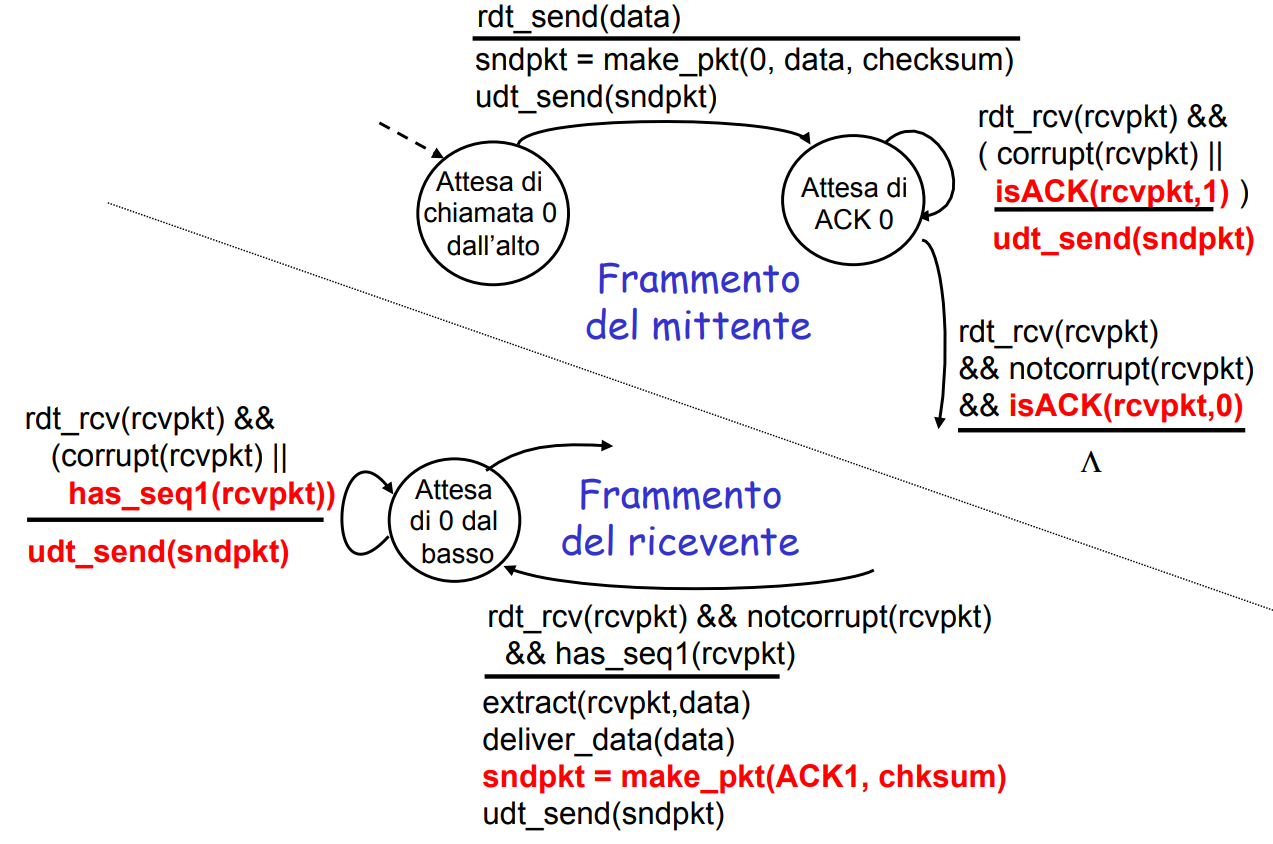
\includegraphics[width=\textwidth]{./img/rdt2.2nonak.png}
\end{center}

Il protocollo \texttt{rdt2.2} elimina l'uso esplicito dei NAK. Il mittente, in attesa di una chiamata dal livello applicativo, crea un pacchetto con numero di sequenza 0 e checksum tramite \texttt{make\_pkt(0, data, checksum)} e lo invia con \texttt{udt\_send(sndpkt)}. 

Il mittente poi attende un ACK. Se riceve un pacchetto corrotto o un ACK con numero di sequenza 1 (tramite \texttt{rdt\_rcv(rcvpkt) \&\& (corrupt(rcvpkt) || isACK(rcvpkt, 1))}), ritrasmette il pacchetto. Se riceve un ACK non corrotto con numero di sequenza 0 (tramite \texttt{rdt\_rcv(rcvpkt) \&\& notcorrupt(rcvpkt) \&\& isACK(rcvpkt, 0)}), torna allo stato di attesa. 

Il destinatario, in attesa di una chiamata dal livello di rete, riceve un pacchetto con \texttt{rdt\_rcv(rcvpkt)}. Se il pacchetto è corrotto o ha il numero di sequenza errato (tramite \texttt{rdt\_rcv(rcvpkt) \&\& (corrupt(rcvpkt) || has\_seq1(rcvpkt))} quando è in attesa di 0 o tramite \texttt{rdt\_rcv(rcvpkt) \&\& (corrupt(rcvpkt) || has\_seq0(rcvpkt))} quando è in attesa di 1), invia un ACK con il numero di sequenza opposto con \texttt{udt\_send(sndpkt)}. Se il pacchetto non è corrotto e ha il numero di sequenza atteso (tramite \texttt{rdt\_rcv(rcvpkt) \&\& notcorrupt(rcvpkt) \&\& has\_seq0(rcvpkt)} quando è in attesa di 0 o tramite \texttt{rdt\_rcv(rcvpkt) \&\& notcorrupt(rcvpkt) \&\& has\_seq1(rcvpkt)} quando è in attesa di 1), estrae i dati con \texttt{extract(rcvpkt,data)}, li consegna al livello applicativo con \texttt{deliver\_data(data)} e invia un ACK con il numero di sequenza atteso con \texttt{udt\_send(sndpkt)}, passando all'altro stato di attesa.

\subsubsection*{RDT3.0: canali con errori e perdite}
Si aggiunge un timer di attesa per la ricezione di un \textbf{ACK}, così in caso di pacchetto perso il mittente ritrasmetterà il pacchetto. Nel caso in cui sia solo il ritardo, il mittente invierà il pacchetto, ma il duplicato verrà gestito tramite i numeri di sequenza.

\begin{center}
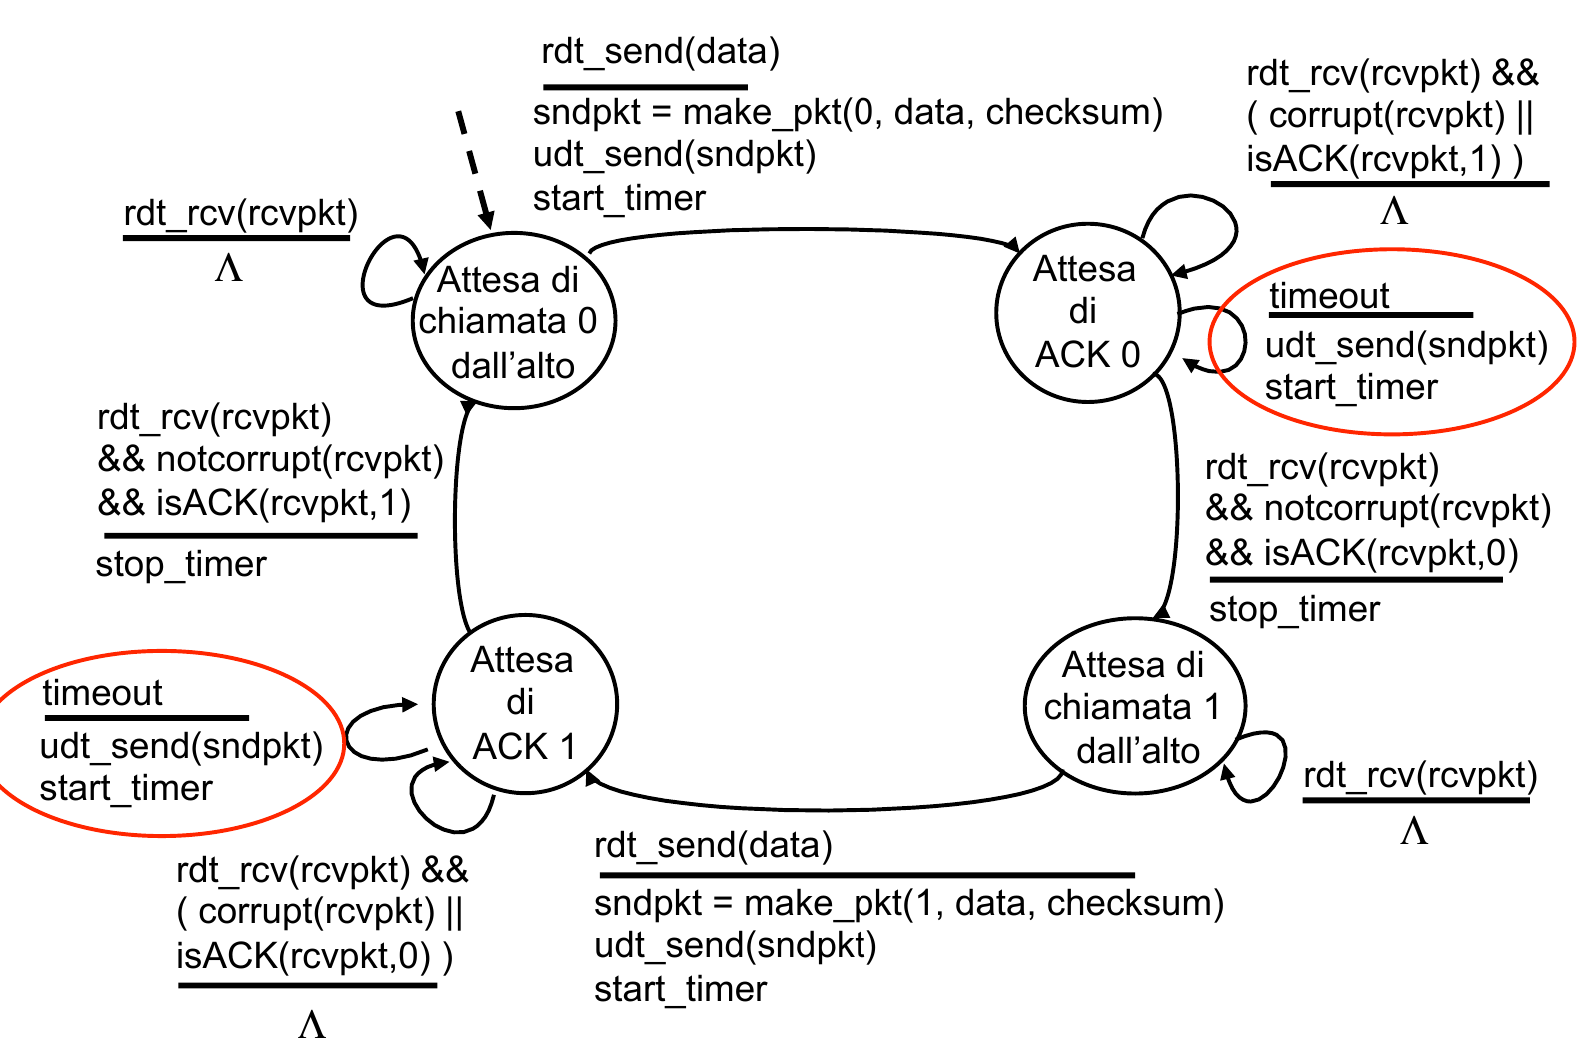
\includegraphics[width=\textwidth]{./img/rdt3.0mit.png}
\end{center}

\begin{quote}
l'automa a stati finiti del ricevente è uguale a quello del \textbf{RTD2.2}
\end{quote}

\subsubsection*{RDT3.0: Perdita di pacchetto}
\begin{center}
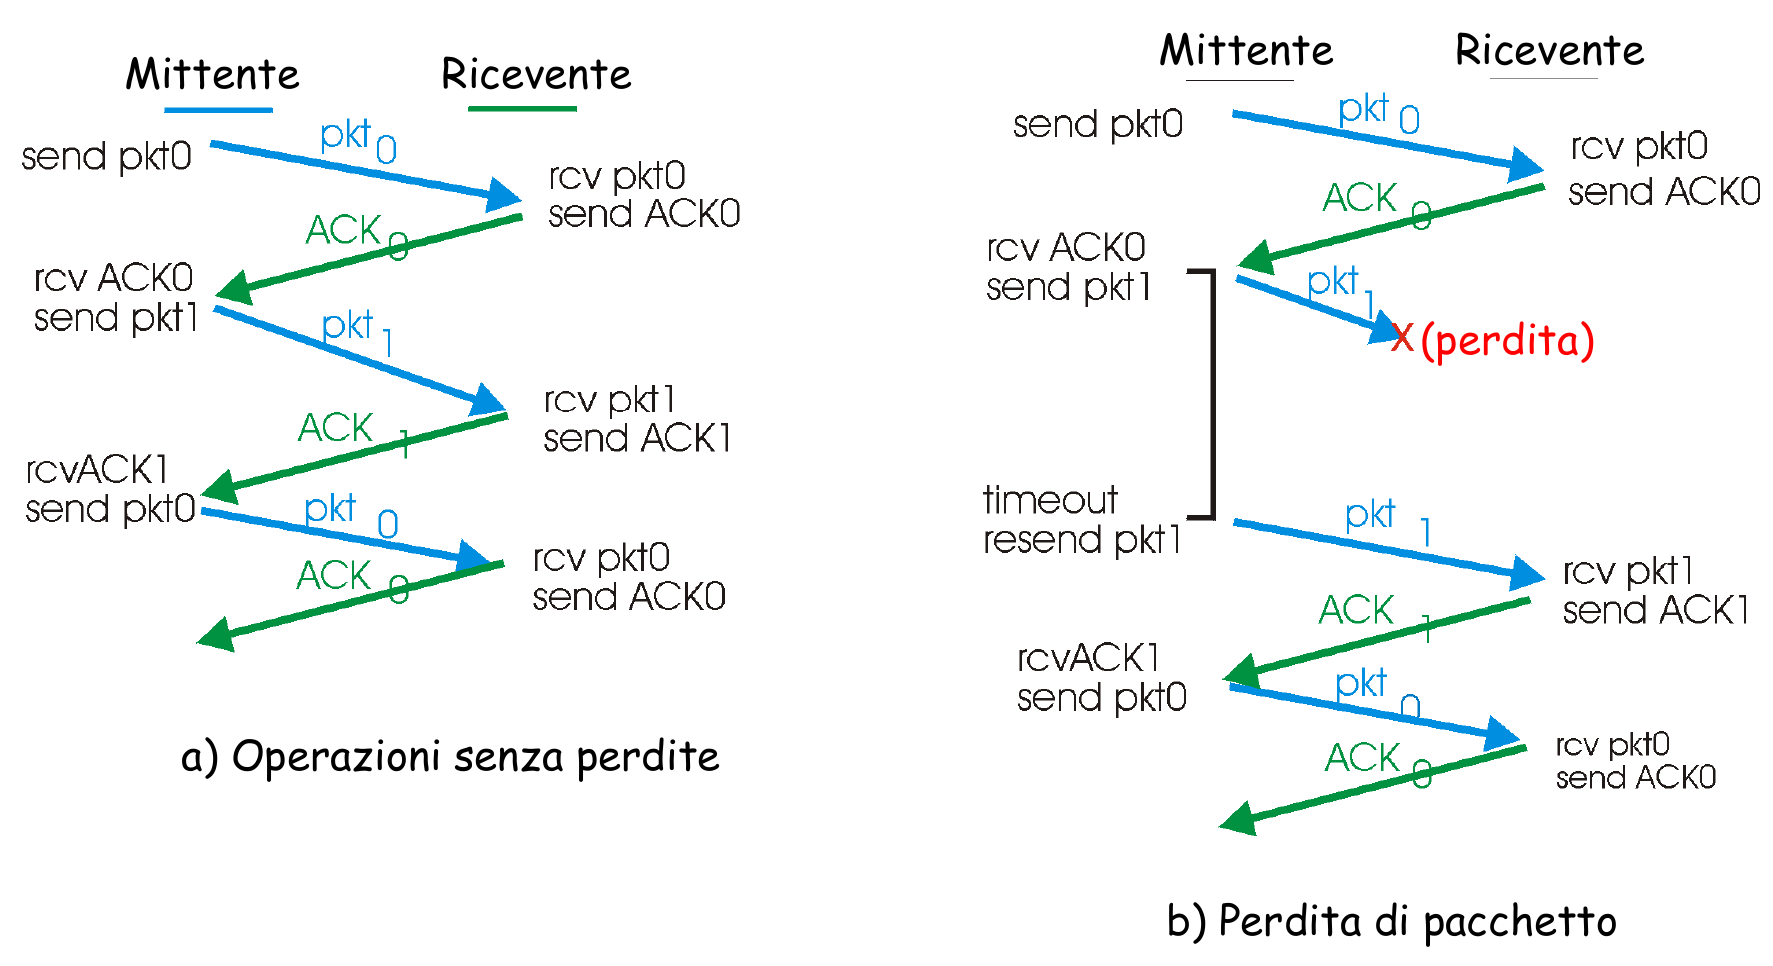
\includegraphics[width=\textwidth]{./img/rdt3.01.png}
\end{center}

\subsubsection*{RDT3.0: Perdita di ACK}
\begin{center}
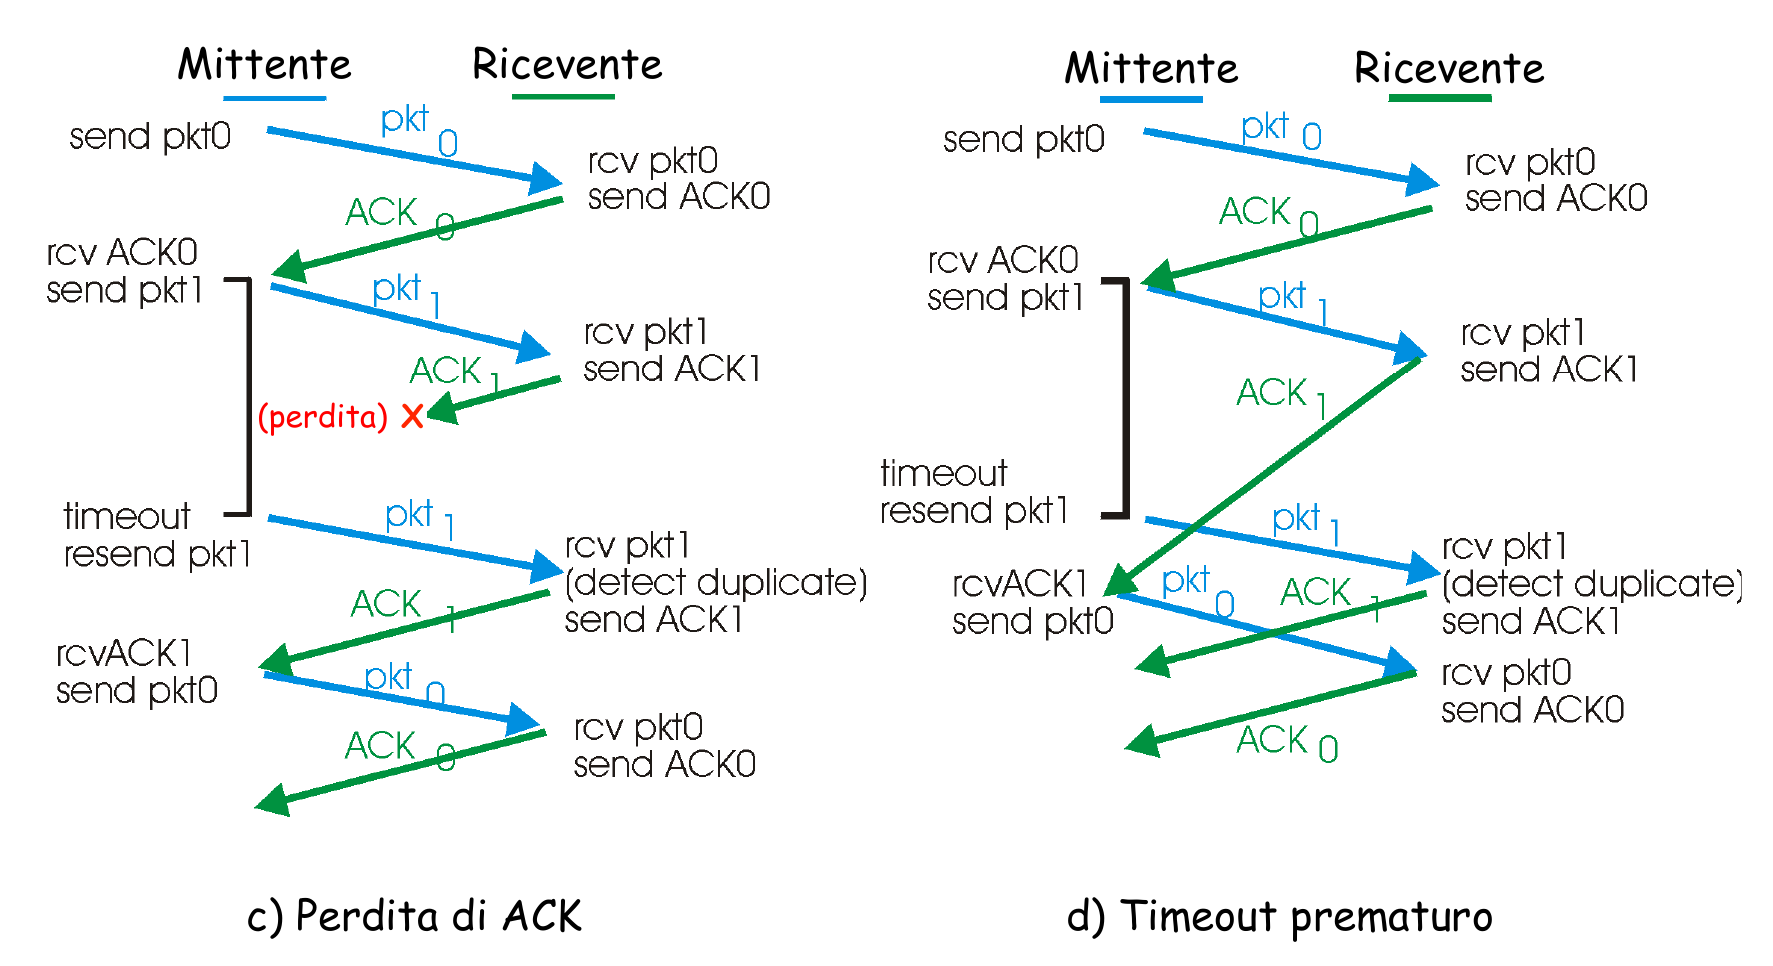
\includegraphics[width=\textwidth]{./img/rdt3.02.png}
\end{center}

Il protocollo \texttt{rdt3.0} introduce un timer per gestire la perdita di pacchetti. Il mittente, in attesa di una chiamata dal livello applicativo, crea un pacchetto con numero di sequenza (0 o 1) e checksum tramite \texttt{make\_pkt(0, data, checksum)} o \texttt{make\_pkt(1, data, checksum)}, lo invia con \texttt{udt\_send(sndpkt)} e avvia un timer con \texttt{start\_timer}. Il mittente poi attende un ACK. Se riceve un pacchetto corrotto o un ACK con numero di sequenza errato (tramite \texttt{rdt\_rcv(rcvpkt) \&\& (corrupt(rcvpkt) || isACK(rcvpkt, 1))} o \texttt{rdt\_rcv(rcvpkt) \&\& (corrupt(rcvpkt) || isACK(rcvpkt, 0))}), ritrasmette il pacchetto e riavvia il timer. Se riceve un ACK non corrotto con il numero di sequenza corretto (tramite \texttt{rdt\_rcv(rcvpkt) \&\& notcorrupt(rcvpkt) \&\& isACK(rcvpkt, 0)} o \texttt{rdt\_rcv(rcvpkt) \&\& notcorrupt(rcvpkt) \&\& isACK(rcvpkt, 1)}), ferma il timer con \texttt{stop\_timer} e passa all'altro stato di attesa. Se il timer scade (tramite \texttt{timeout}), ritrasmette il pacchetto e riavvia il timer. Il ricevente ha lo stesso automa a stati finiti del protocollo \texttt{rdt2.2}.

Il \textbf{RDT3.0} utilizza un algoritmo \textbf{STOP and WAIT} ma è molto lento, utilizziamo le \textbf{pipeline} per velocizzare il sistema.

\subsubsection{Protocolli con pipeline}
Utilizzeremo due tipi di meccanismi, sono opposti come filosofia.

\subsubsection{Go-Back-N}
\begin{itemize}
  \item Il mittente può avere fino a $N$ pacchetti senza ACK in pipeline (finestra scorrevole).
  \item Il ricevente ha un buffer di dimensione 1 e mantiene solo il numero di sequenza atteso.
  \item Il ricevente invia solo \textbf{ACK cumulativi}, non dà l'ACK di un pacchetto se c'è un gap.
  \item Il mittente ha un singolo timer per il pacchetto base della finestra (il più vecchio non riscontrato). Quando arriva un ACK per questo pacchetto, il timer viene riavviato per il nuovo pacchetto base.
\end{itemize}

L'ACK sarà con il numero di sequenza dell'ultimo pacchetto arrivato correttamente e in ordine. Il mittente può continuare a mandare altri pacchetti, ma quelli con numero di sequenza superiore a quello atteso vengono scartati dal ricevitore, che continua a mandare ACK per l'ultimo pacchetto ricevuto correttamente in ordine.

\begin{center}
  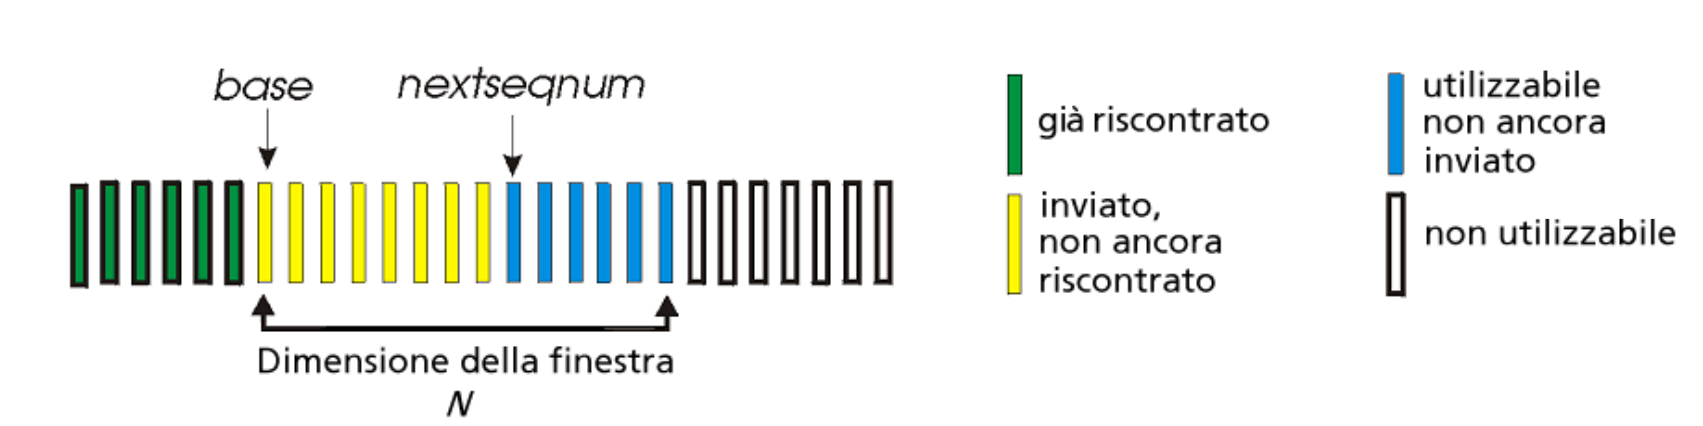
\includegraphics[width=\textwidth]{./img/gobackn.png}
\end{center}

La finestra contiene $N$ pacchetti inviati di cui ancora non è arrivato un riscontro e scorre in avanti quando vengono ricevuti gli ACK.
nextseqnum: prossimo pacchetto da inviare.
Il protocollo Go-Back-N (GBN) permette al mittente di inviare fino a $N$ pacchetti senza attendere un ACK per ognuno. Il ricevente invia solo ACK cumulativi, confermando la ricezione di tutti i pacchetti fino a un certo numero di sequenza. Se il mittente non riceve un ACK entro un certo tempo, ritrasmette tutti i pacchetti non ancora confermati. Come si vede nell'immagine, il mittente mantiene una finestra di $N$ pacchetti inviati ma non ancora confermati, e il puntatore \textit{nextseqnum} indica il prossimo pacchetto da inviare.

\subsubsection*{Go-Back-N: Funzionamento passo per passo}

\begin{enumerate}
  \item \textbf{Invio Pacchetti:} Il mittente invia pacchetti con numeri di sequenza crescenti (0, 1, 2, ...), fino a raggiungere la dimensione massima della finestra $N$.
  \item \textbf{Ricezione ACK Cumulativi:} Il ricevente invia ACK cumulativi, confermando la ricezione di tutti i pacchetti fino a un certo numero di sequenza. Ad esempio, un ACK con numero di sequenza 3 indica che i pacchetti 0, 1, 2 e 3 sono stati ricevuti correttamente.
  \item \textbf{Gestione Buffer Ricevitore:} Il ricevitore mantiene un singolo numero di sequenza atteso. Tutti i pacchetti con numero di sequenza superiore vengono immediatamente scartati.
  \item \textbf{Timeout e Ritrasmissione:} Il mittente mantiene un timer per il pacchetto con il numero di sequenza più basso non ancora confermato. Se il timer scade, il mittente ritrasmette tutti i pacchetti non ancora confermati, a partire dal pacchetto con il numero di sequenza più basso.
  \item \textbf{Esempio di funzionamento senza perdite:}
  \begin{enumerate}
    \item Il mittente invia i pacchetti 0, 1 e 2.
    \item Il ricevente riceve i pacchetti 0, 1 e 2 e invia un ACK con numero di sequenza 2.
    \item La finestra del mittente scorre in avanti e il mittente invia i pacchetti 3, 4 e 5.
  \end{enumerate}

  \item \textbf{Esempio di funzionamento con perdita di pacchetto:}
  \begin{enumerate}
    \item Il mittente invia i pacchetti 0, 1 e 2.
    \item Il pacchetto 1 viene perso.
    \item Il ricevente riceve il pacchetto 0 e poi il pacchetto 2, ma scarta il pacchetto 2 perché attende il pacchetto 1. Continua a inviare ACK per il pacchetto 0.
    \item Il timer del mittente per il pacchetto 0 scade.
    \item Il mittente ritrasmette i pacchetti 0, 1 e 2.
    \item Il ricevente riceve i pacchetti 0, 1 e 2 e invia un ACK con numero di sequenza 2.
  \end{enumerate}
\end{enumerate}

\subsubsection{Selective Repeat}
Il protocollo Selective Repeat (SR) permette al ricevente di inviare ACK per ogni pacchetto ricevuto correttamente, anche se non sono in ordine. A differenza del Go-Back-N, il ricevitore mantiene un buffer per i pacchetti fuori sequenza. La dimensione della finestra deve essere minore o uguale a $N/2$, dove $N$ è la dimensione dello spazio dei numeri di sequenza, per evitare ambiguità nella numerazione dei pacchetti.

Il mittente mantiene un timer per ogni pacchetto inviato e ritrasmette solo i pacchetti per cui non ha ricevuto un ACK entro il timeout. Come si vede nell'immagine, il ricevente può accettare e bufferizzare pacchetti anche se non sono in ordine, e il mittente ritrasmette solo i pacchetti persi.

\begin{center}
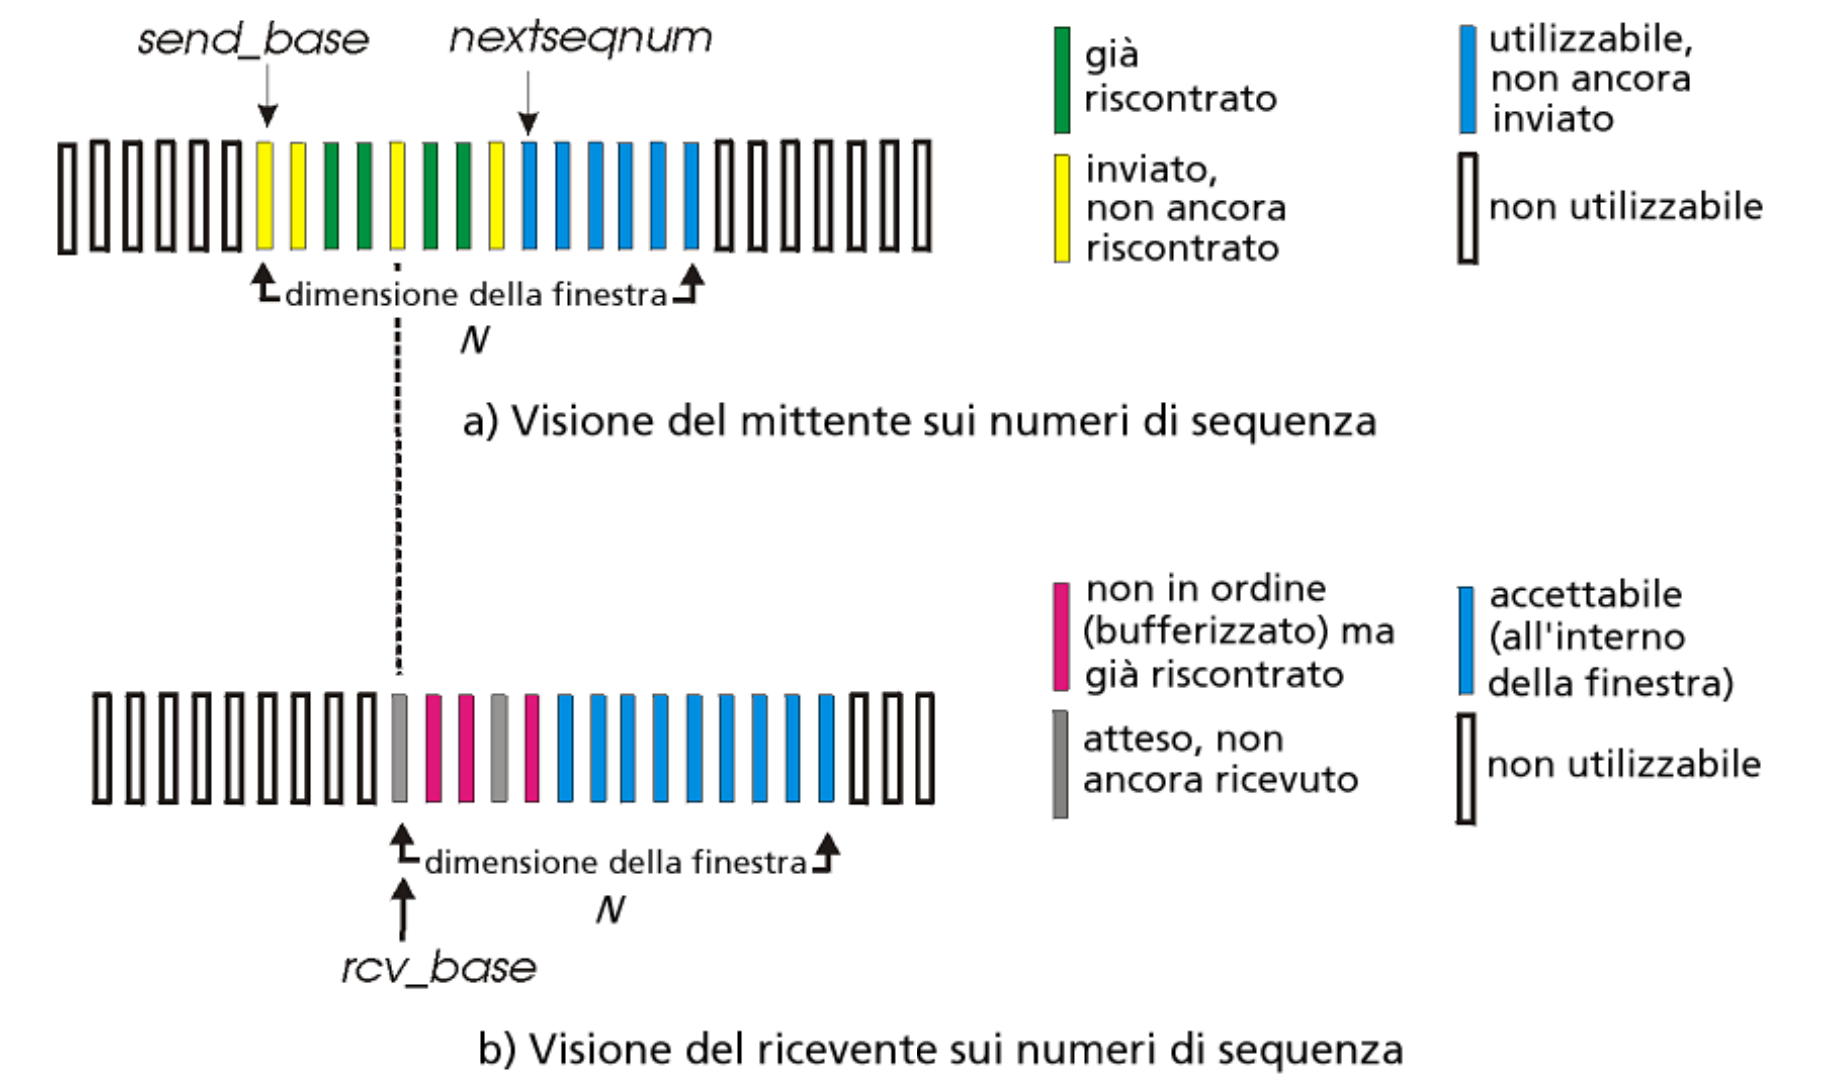
\includegraphics[width=\textwidth]{./img/ripetizioneselettiva.png}
\end{center}

\subsubsection*{Selective Repeat: funzionamento passo per passo}
\begin{enumerate}
  \item \textbf{Invio Pacchetti:} Il mittente invia pacchetti con numeri di sequenza crescenti (0, 1, 2, ...), fino a raggiungere la dimensione massima della finestra ($\le N/2$).
  \item \textbf{Ricezione ACK Selettivi:} Il ricevente invia ACK selettivi, confermando la ricezione di ogni singolo pacchetto.
  \item \textbf{Gestione Buffer Ricevitore:}
  \begin{itemize}
    \item Il ricevitore mantiene un buffer per i pacchetti fuori sequenza
    \item I pacchetti vengono bufferizzati fino a quando possono essere consegnati in ordine al livello superiore
    \item La consegna al livello superiore avviene solo quando tutti i pacchetti precedenti sono stati ricevuti
  \end{itemize}
  \item \textbf{Timeout e Ritrasmissione Selettiva:} Il mittente mantiene un timer per ogni pacchetto inviato. Se il timer di un pacchetto scade, il mittente ritrasmette solo quel pacchetto.
  
  \item \textbf{Esempio di funzionamento senza perdite:}
  \begin{enumerate}
    \item Il mittente invia i pacchetti 0, 1 e 2.
    \item Il ricevente riceve i pacchetti 0, 1 e 2 e invia ACK per ognuno di essi.
    \item I pacchetti vengono consegnati in ordine al livello superiore.
    \item Il mittente riceve gli ACK e invia i pacchetti 3, 4 e 5.
  \end{enumerate}
  \item \textbf{Esempio di Funzionamento con Perdita di Pacchetto:}
  \begin{enumerate}
       \item Il mittente invia i pacchetti 0, 1 e 2 (assumiamo finestra di dimensione 3).
       \item Il pacchetto 1 viene perso.
       \item Il ricevente riceve i pacchetti 0 e 2:
           \begin{itemize}
               \item Invia ACK per 0 e ACK per 2
               \item Bufferizza il pacchetto 2 (fuori sequenza)
           \end{itemize}
       \item Il mittente riceve ACK 0:
           \begin{itemize}
               \item La sua finestra scorre in avanti di una posizione
               \item Avendo spazio nella finestra (che ora contiene 1[non ACKed], 2, \_), invia il pacchetto 3
               \item Il pacchetto 1 rimane nella finestra come non riscontrato
           \end{itemize}
       \item Il mittente riceve ACK 2:
           \begin{itemize}
               \item Marca il pacchetto 2 come riscontrato nella finestra
               \item La finestra ora contiene (1[non ACKed], 2[ACKed], 3)
               \item Avendo spazio nella finestra per un nuovo pacchetto, invia il pacchetto 4
           \end{itemize}
       \item Il timer del pacchetto 1 scade:
           \begin{itemize}
               \item Il mittente ritrasmette solo il pacchetto 1
               \item Continua a gestire normalmente il resto della finestra (pacchetti 2, 3, 4)
           \end{itemize}
       \item Il ricevente riceve il pacchetto 1:
           \begin{itemize}
               \item Invia un ACK per 1
               \item Ora può consegnare in ordine i pacchetti 0, 1 e 2 al livello superiore
           \end{itemize}
       \item Il mittente riceve ACK 1:
           \begin{itemize}
               \item La finestra scorre ancora (ora contiene 3, 4, \_)
               \item Invia il pacchetto 5 nello spazio disponibile
           \end{itemize}
  \end{enumerate}
\end{enumerate}

\textbf{THROUGHPUT}: tasso di occupazione medio con cui i dati vengono trasmessi sul collegamento, rapporto tra tutti i dati trasmessi (anche più volte). \

\textbf{GOODPUT}: tasso con cui il livello applicativo di destinazione vede arrivare i dati utili, rapporto tra i dati utili e il tempo di trasmissione. \

Il \textit{throughput} è sempre maggiore del \textit{goodput}, solo nel caso ideale saranno uguali.

\subsection{TCP: trasporto orientato alla connessione}
È un tipo di connessione \textbf{punto-punto}, ovvero una connessione \textit{logica} tra mittente e destinatario, \textbf{full duplex}, abbiamo un flusso di dati bidirezionale, ovvero i dati possono fluire in \textit{entrambe le direzioni simultaneamente}, e \textbf{orientato alla connessione}, ovvero TCP usa un \textit{handshaking a tre vie} per stabilire la connessione, ha un flusso di byte affidabile, ovvero TCP garantisce la consegna dei dati nell'ordine corretto.
I dati vengono mandati in \textbf{pipeline}, ovvero TCP permette di avere \textit{più segmenti} in transito simultaneamente, attraverso un meccanismo \textit{sliding window}, usato per il \textit{controllo di flusso} e il \textit{controllo di congestione}, abbiamo un \textbf{buffer d'invio} e un \textbf{buffer di ricezione}, usati per \textit{memorizzare i dati} prima della trasmissione e dopo la ricezione, così che i pacchetti che arrivano fuori ordine vengono conservati e riordinati successivamente.

\subsubsection{Struttura dei segmenti}

\textbf{L'OVERHEAD} minimo del \textit{TCP} è di \textbf{20 Byte}, ma l'header TCP ha una lunghezza \textit{variabile} a causa del campo opzioni.
\begin{itemize}
  \item Prima riga - uguale alla struttura del protocollo \textit{UDP}, serve per il \textit{multiplexing e demultiplexing}.
  \item Seconda riga - \textbf{Numero di sequenza}: Posizione del primo Byte all'interno del payload (= MSS, Maximum Segment Size).
  \item Terza riga - \textbf{Numero di riscontro}: Il numero di riscontro sarà il \textit{prossimo numero di sequenza atteso}, ovvero il primo byte del segmento successivo a quello arrivato.
  \item Quarta riga - \textbf{BIT DI FLAG}: U (dati urgenti), A (\textbf{ACK}), P (PUSH), R (RST), S (SYN), F (FIN), gli ultimi tre sono comandi per impostare e chiudere la connessione, questi bit sono usati per la \textit{gestione della connessione} e il \textit{controllo di flusso}.
  \item Quarta riga - \textbf{Lunghezza intestazione}: nel protocollo UDP è sempre 8 byte, qui no, verrà specificato pacchetto per pacchetto, indicando la lunghezza dell'header in \textit{parole di 32 bit}.
  \item Quarta riga - \textbf{Finestra di ricezione}: Da non confondere con la \textit{sliding window}, dice quanto spazio si ha a disposizione per ricevere i dati, usata per il \textit{controllo di flusso} e indica la \textit{quantità di dati} che il ricevitore è disposto ad accettare.
  \item Quinta riga - \textbf{checksum}: grandezza di 16 bit, calcolata come la checksum dell'UDP, ovvero sull'\textit{intero segmento TCP}, inclusi header e dati.
  \item Quinta riga - \textbf{Puntatore ai dati urgenti}: Nel caso in cui la flag U sia attiva ci sarà il puntatore alla memoria per quei dati, indicando la \textit{fine dei dati urgenti}.
  \item Sesta riga - \textbf{Opzioni}: varie ed eventuali, usate per \textit{funzionalità opzionali} come il timestamping.
\end{itemize}

\begin{center}
  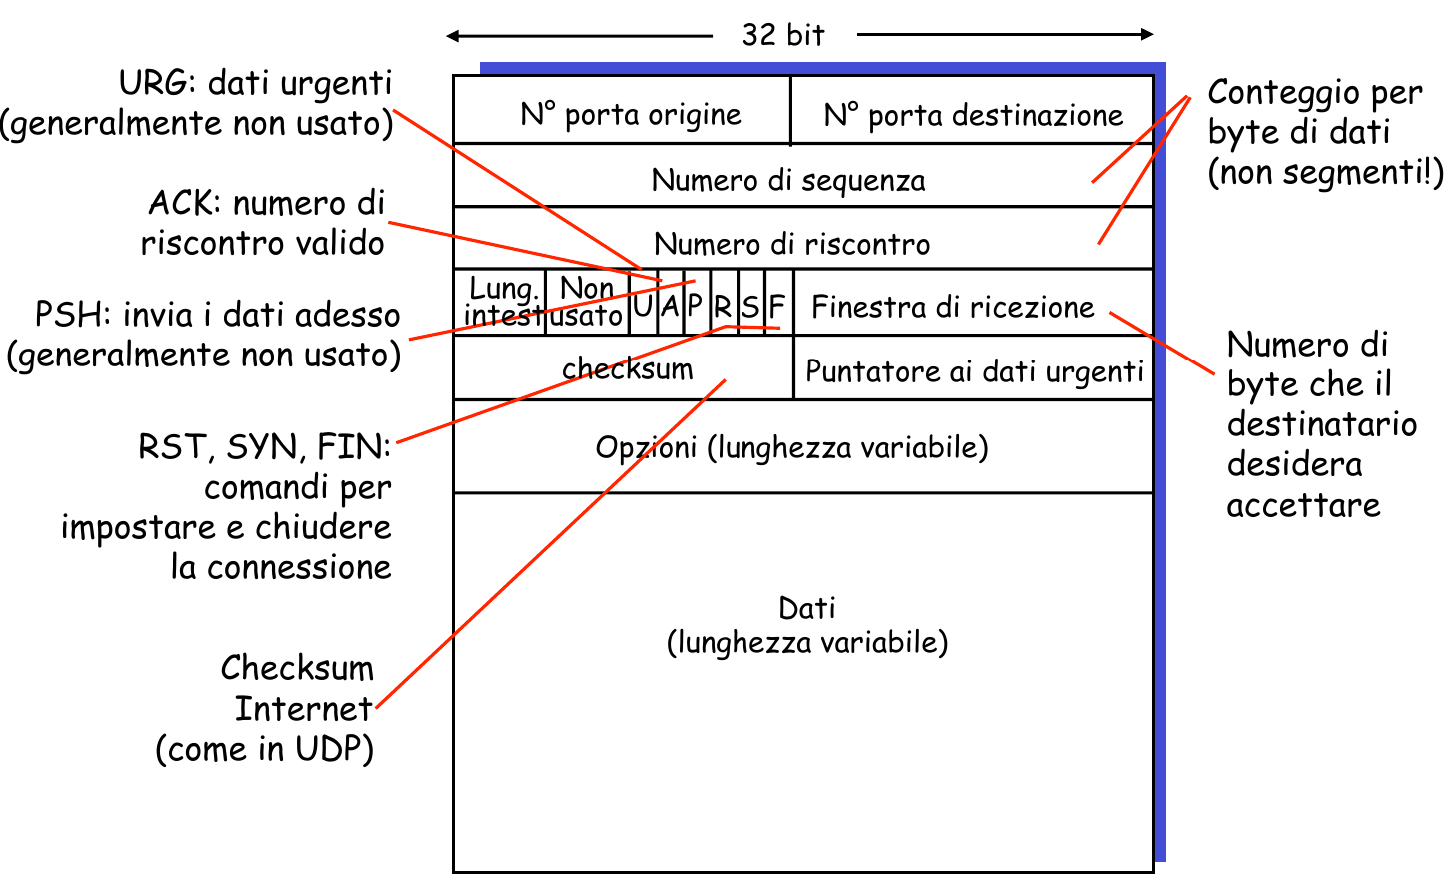
\includegraphics[width=\textwidth]{img/segmento_tcp.png}
\end{center}

\subsubsection{Gestione numeri di sequenza e riscontro del TCP}
Il \textit{numero di sequenza} è il numero di byte nel flusso di dati che corrisponde al primo byte di dati nel segmento, dipende dal mittente e da come gestisce la memoria del proprio \textbf{buffer di invio}.
Il \textit{numero di riscontro} utilizza un \textit{ACK cumulativo}, sarà il numero del prossimo byte che il destinatario si aspetta di ricevere in ordine, quindi sarà il primo byte del segmento che vorrà ricevere, quindi del successivo all'ultimo correttamente ricevuto e immagazzinato, dipende dal destinatario e da come gestisce la memoria del proprio \textbf{buffer di ricezione}.

\begin{center}
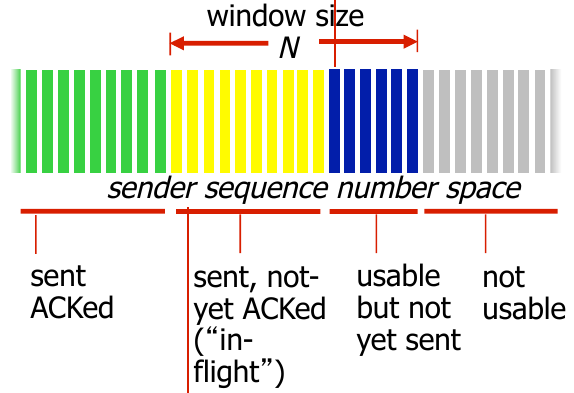
\includegraphics[width=\textwidth]{./img/tcpseqack.png}
\end{center}

\subsubsection{Gestione del timer nel TCP}
Il problema principale è stimare correttamente la durata del timer utilizzando la \textbf{media mobile esponenziale ponderata}. L'obiettivo è impostare un timeout \textit{ragionevole}, che non sia troppo corto (causando ritrasmissioni inutili) né troppo lungo (causando ritardi). La media mobile esponenziale ponderata è una tecnica che dà \textit{più peso ai campioni recenti} del RTT. La formula è la seguente:
\[
\text{EstimatedRTT}(t) = (1 - \alpha) \cdot \text{EstimatedRTT}(t-1) + \alpha \cdot \text{SampleRTT}(t)
\]
dove solitamente \(\alpha = 0.125\). In questa formula, `EstimatedRTT(t-1)` è il RTT stimato \textit{precedente} e `SampleRTT(t)` è il RTT misurato \textit{corrente}.
Bisogna calcolare la \textit{deviazione standard} del RTT:
\[
  \text{DevRTT}(t) = (1 - \beta) \cdot \text{DevRTT}(t-1) + \beta \cdot \lvert \text{SampleRTT} - \text{EstimatedRTT}\rvert
\]
dove solitamente \(\beta = 0.25\). In questa formula, `DevRTT(t-1)` è la deviazione stimata \textit{precedente} e `$\lvert$SampleRTT - EstimatedRTT$\rvert$` è la \textit{differenza assoluta} tra il RTT misurato e quello stimato.
\[\text{TimeoutInterval} = \text{EstimatedRTT} + 4 \cdot \text{DevRTT}\]
Il timeout è calcolato aggiungendo un \textit{multiplo della deviazione} al RTT stimato.

\subsubsection{Trasferimento dati affidabile del TCP}
\subsubsection*{Eventi del mittente}
Il \textit{livello di trasporto} riceve i dati dal \textit{livello applicativo}, crea i pacchetti e aggiunge all'intestazione la checksum a ogni pacchetto. Il mittente mantiene un \textbf{buffer di invio} per memorizzare i dati non ancora confermati. Invia il pacchetto al destinatario che ricalcolerà il checksum e controllerà se è corretto.
In caso di timeout o di \textit{ACK} duplicati, che indicano una \textit{potenziale perdita} di un segmento, il protocollo TCP ritrasmetterà il pacchetto, riavviando il timer. Il timeout è associato al \textit{segmento non ancora riscontrato più vecchio}.
Controlla gli \textit{ACK} ricevuti, aggiorno ciò che è stato ricevuto e avvio il time nel caso in cui dovessi completare segmenti già inviati.

\begin{lstlisting}
NextSeqNum = InitialSeqNum
SendBase = InitialSeqNum
loop (sempre) {
  switch (evento)

  evento: i dati ricevuti dall'applicazione superiore
    creano il segmento TCP con numero di sequenza NextSeqNum
    if (il timer attualmente non funziona)
      avvia il timer
    passa il segmento a IP
    NextSeqNum = NextSeqNum + lunghezza(dati)

  evento: timeout del timer
    ritrasmetti il segmento non ancora riscontrato con il piu' piccolo numero di sequenza
  
  evento: ACK ricevuto con valore del campo ACK y
    if (y > SendBase) {
      SendBase = y
      if (esistono timer non attualmente riscontrati)
        avvia timer
    }
} /* fine loop */
\end{lstlisting}
Quando si ritrasmette il pacchetto, il protocollo raddoppia il tempo di timeout al riavvio, nel caso di altra ritrasmissione raddoppierà il valore dell'ultimo timeout usato (quindi già raddoppiato). Questo è un meccanismo di \textit{evitamento della congestione}.

\subsubsection*{Algoritmo della ritrasmissione rapida}
Quando si arriva a 3 ACK duplicati si effettua una ritrasmissione rapida, prima che scada il timer. La ritrasmissione rapida è un meccanismo di \textit{controllo della congestione} che aiuta a evitare ritardi inutili, il timer non viene spento.
Nel caso in cui nel frattempo sono arrivati i pacchetti successivi, il destinatario, al momento in cui riceverà il pacchetto che era andato perso e per cui ha mandato 3 ACK duplicati, invierà l'ACK del successivo dell'ultimo pacchetto ricevuto (sono stati bufferizzati nel mentre che aspettava quel pacchetto).

\begin{lstlisting}
evento:  ACK ricevuto, con valore del campo ACK pari a y
  if (y > SendBase) {
    SendBase = y 
  if (esistono attualmente segmenti non ancora riscontrati)
  avvia il timer
  } else {
    incrementa il numero di ACK duplicati ricevuti per y
    if (numero di ACK duplicati ricevuti per y = 3) {
      rispedisci il segmento con numero di sequenza y
  }
\end{lstlisting}

\subsubsection{Controllo del flusso}
Ricordiamoci che il protocollo \textit{TCP} inizializza delle zone di memoria per il \textit{buffer di ricezione} e \textit{buffer di invio}, che si trovano nei \textit{sistemi terminali}, il mittente non deve sovraccaricare il buffer del destinatario. 

Il controllo di flusso serve a \textit{prevenire che il mittente sovraccarichi il ricevitore}.

Mittente e destinatario comunicano continuamente quanto spazio hanno libero nei vari buffer.

Il valore di \textbf{RcvWindow} verrà inserito all'interno dei segmenti, il mittente usa il valore di `RcvWindow` per \textit{limitare la quantità di dati non riscontrati} che invia, così che non vengano inviati dati che verranno sicuramente persi. Il campo `RcvWindow` indica la \textit{quantità di spazio libero} nel buffer del ricevitore.
\textbf{RcvBuffer} funzione per la creazione della socket, è una \textit{system call} usata per impostare la dimensione del buffer di ricezione.

\begin{center}
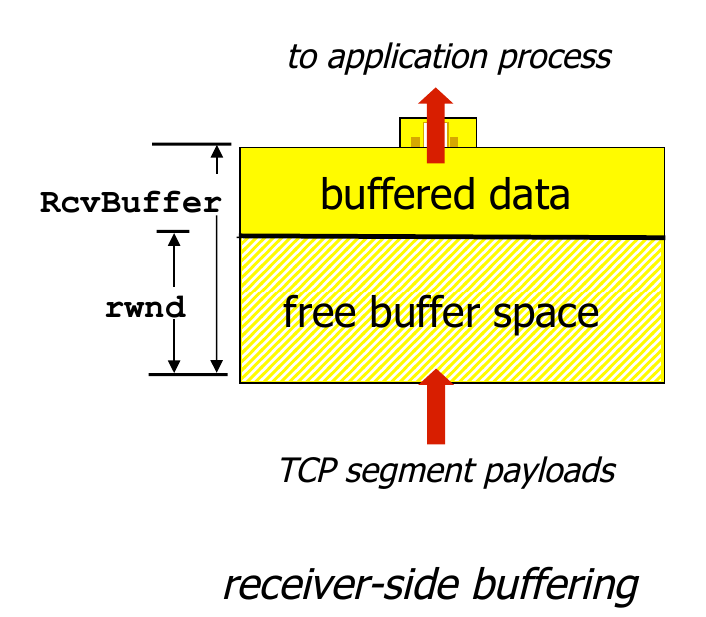
\includegraphics[width=0.3\textwidth]{./img/tcpflowcontrol.png}
\end{center}

L'immagine mostra il buffer di ricezione lato destinatario. Il buffer è diviso in due parti: la parte superiore, dove sono memorizzati i dati ricevuti ma non ancora consegnati all'applicazione, e la parte inferiore, che rappresenta lo spazio libero nel buffer. Il valore \textit{RcvWindow} (indicato come \textit{rwnd} nell'immagine) indica la dimensione dello spazio libero nel buffer di ricezione, e viene comunicato al mittente per regolare la velocità di trasmissione.

\subsubsection*{Gestione della connessione: Handshake a tre vie}
Si stabilisce una connessione tra mittente e destinatario, si mettono d'accordo e inizializzano dei dati come \textit{numero di sequenza} e i \textit{buffer}.
L'inizializzazione della connessione avviene tramite l'\textbf{Handshake a tre vie}:
\begin{itemize}
  \item Passo 1: il client invia un segmento SYN al server \\
      specifica il numero di sequenza iniziale, scelto in modo casuale \\
      nessun dato
  \item Passo 2:  il server riceve SYN e risponde con un segmento SYNACK \\
      il server alloca i buffer \\
      specifica il numero di sequenza iniziale del server, scelto in modo casuale \\
      il segmento SYNACK ha il flag SYN e ACK impostati a 1
  \item Passo 3:  il client riceve SYNACK e risponde con un segmento ACK, che può contenere dati \\
      il segmento ACK ha il flag ACK impostato a 1
\end{itemize}

\begin{center}
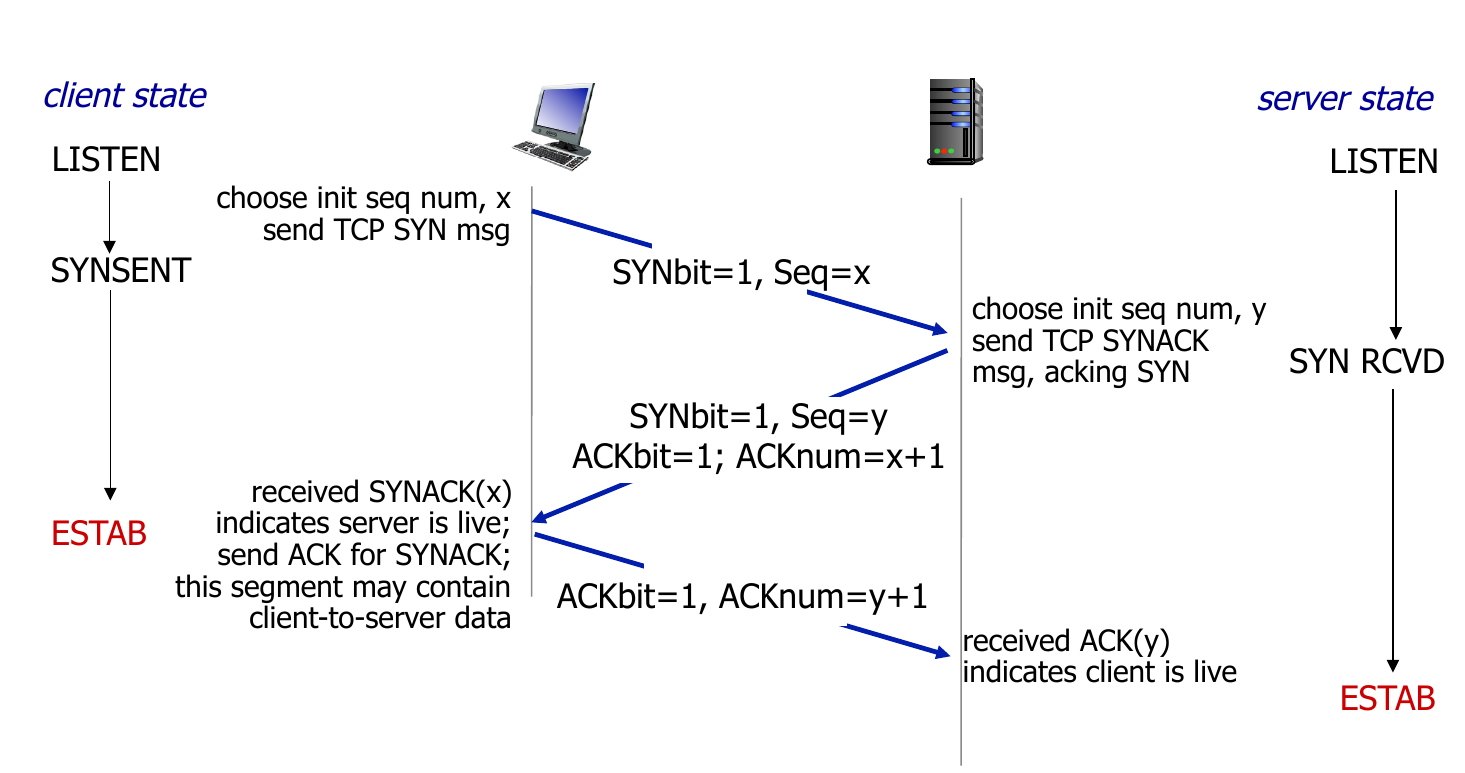
\includegraphics[width=\textwidth]{./img/handshake3vie.png}
\end{center}

Per chiudere una connessione abbiamo 4 passi:
\begin{itemize}
  \item Passo 1: il \textit{client} invia un segmento di controllo FIN al server, con il flag FIN impostato a 1.
  \item Passo 2: il \textit{server} riceve il segmento FIN e risponde con un ACK e invia un FIN.
  \item Passo 3: il \textit{client} riceve FIN e risponde con un ACK. Inizia l’attesa temporizzata - risponde con un ACK ai FIN che riceve.
  \item Passo 4: il \textit{server} riceve un ACK. La connessione viene chiusa.
\end{itemize}

\begin{center}
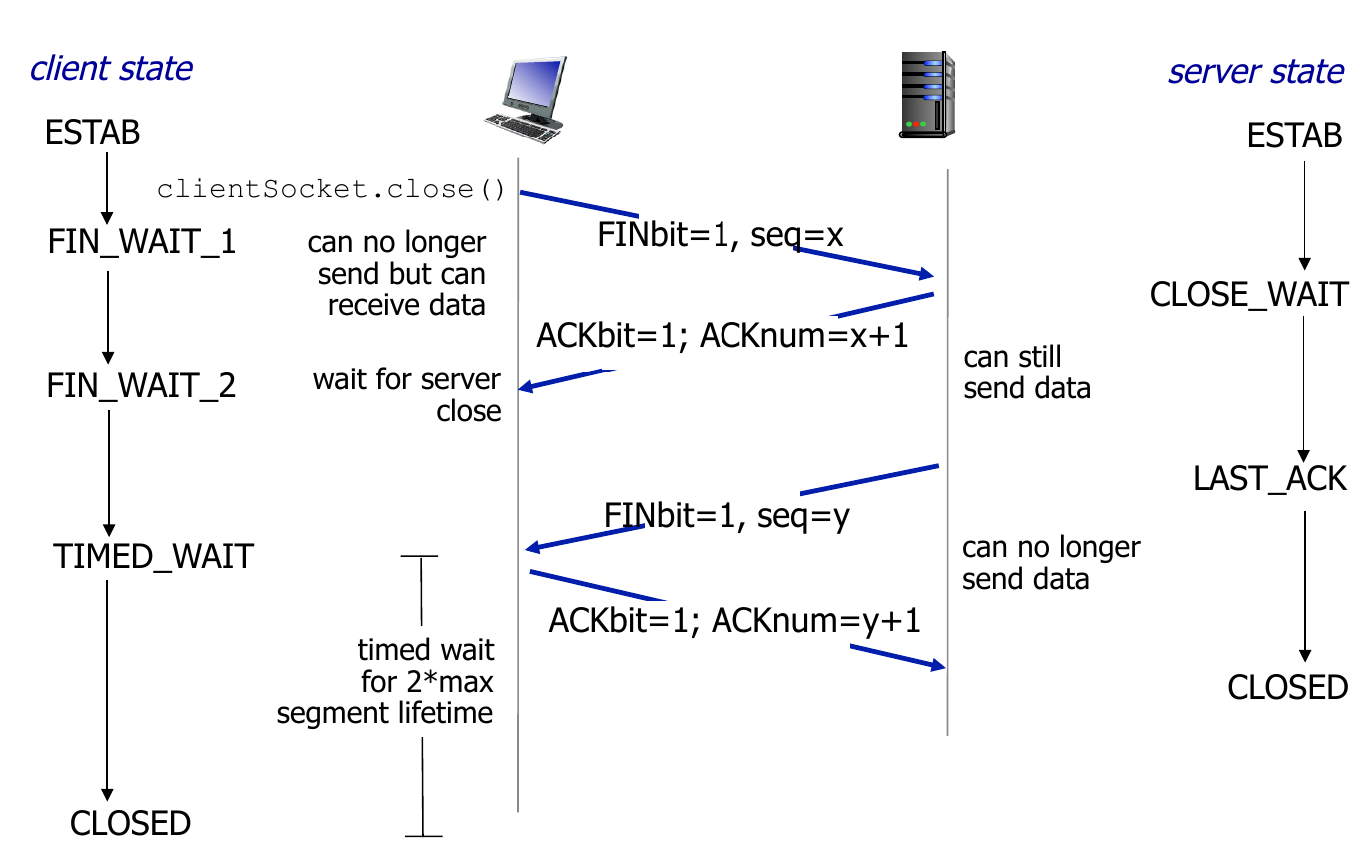
\includegraphics[width=\textwidth]{./img/chiusuraconnessionetcp.png}
\end{center}
Il client entra in uno stato di attesa temporizzata dopo aver inviato l'ultimo ACK per assicurarsi che il server abbia ricevuto l'ACK e che eventuali segmenti in ritardo vengano gestiti correttamente.

\subsection{Principi del controllo di congestione}
La \textbf{congestione} è il blocco della rete per via di un numero di dati elevato mandati a una velocità elevata che la \textit{rete} non riesce a gestirli, ovvero quando le \textit{risorse di rete sono sovraccariche}.
Ciò causa pacchetti smarriti (overflow nel buffer) e lunghi ritardi (di accodamento nei buffer), che possono \textit{degradare le prestazioni della rete}. La congestione è causata da \textit{più mittenti} che trasmettono dati ad alta velocità.

\subsubsection*{Scenario di Congestione 1: Due Mittenti e Buffer Illimitati}
In questo scenario, due mittenti inviano dati a due destinatari attraverso un singolo router con buffer illimitati e un collegamento condiviso di capacità R. Non ci sono ritrasmissioni.

\begin{center}
  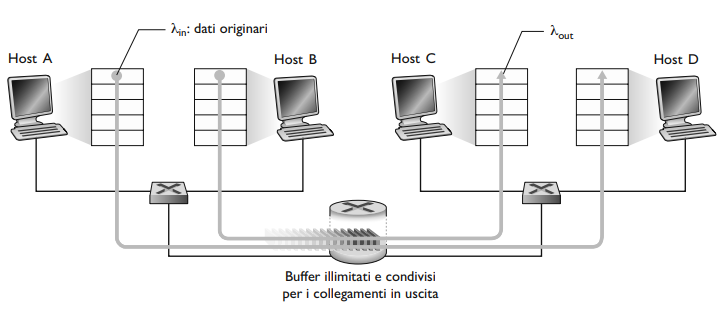
\includegraphics[width=\textwidth]{img/scenario1.png}
\end{center}

\begin{itemize}
    \item \textbf{Throughput:} Quando il tasso di invio combinato (\(\lambda_{in}\)) è inferiore a R/2, il throughput per connessione è uguale al tasso di invio. Quando il tasso di invio combinato supera R/2, il throughput per connessione è limitato a R/2.
    \item \textbf{Ritardo:} Quando il tasso di invio si avvicina a R/2, il ritardo medio aumenta. Quando si arriva ad esser molto vicini a R/2 il ritardo medio tende all'infinito a causa dell'accodamento illimitato.
\end{itemize}
\textbf{Conclusione:} Anche in uno scenario idealizzato con buffer illimitati, la congestione causa ritardi significativi quando il tasso di invio si avvicina alla capacità del collegamento, nonostante si raggiunga il throughput massimo.

\subsubsection*{Scenario di Congestione 2: Buffer Finiti e Ritrasmissioni}
In questo scenario, si considera un router con buffer di dimensione limitata. I pacchetti che arrivano in un buffer pieno vengono scartati, e i mittenti ritrasmettono i pacchetti persi.

\begin{center}
  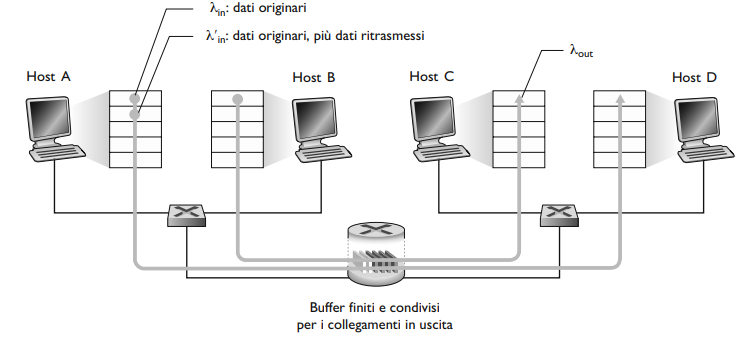
\includegraphics[width=\textwidth]{img/scenario2.png}
\end{center}

\begin{itemize}
    \item \textbf{Caso a) Ritrasmissione "Magica":} Il mittente trasmette solo quando il buffer ha spazio. In questo caso, non ci sono perdite, \(\lambda'_{in} = \lambda_{in}\), e il throughput è \(\lambda_{in}\) fino a R/2.
    \item \textbf{Caso b) Ritrasmissione Perfetta:} Il mittente ritrasmette solo quando è certo che un pacchetto sia andato perso. In questo caso, \(\lambda'_{in} > \lambda_{out}\), e il throughput è R/3 quando il carico offerto (\(\lambda'_{in}\)) è R/2.
    \item \textbf{Caso c) Ritrasmissione Prematura:} Il mittente può andare in timeout prematuramente e ritrasmettere un pacchetto che non è stato perso. In questo caso, il throughput è R/4 quando il carico offerto (\(\lambda'_{in}\)) è R/2, a causa di ritrasmissioni non necessarie.
\end{itemize}

\begin{center}
  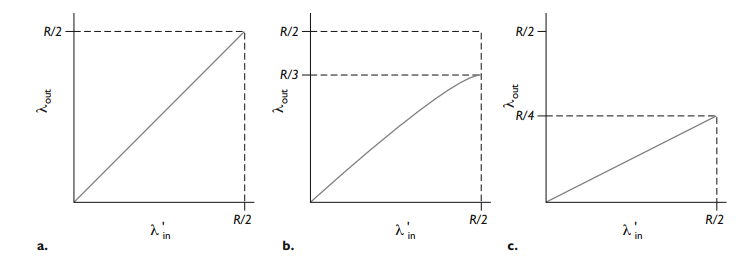
\includegraphics[width=\textwidth]{img/scenario2diag.png}
\end{center}

\textbf{Costi della Congestione:}
\begin{itemize}
    \item Più lavoro (ritrasmissioni) per un dato \textit{goodput}.
    \item Ritrasmissioni non necessarie: il collegamento trasporta più copie dello stesso pacchetto.
\end{itemize}

\subsubsection*{Scenario di Congestione 3: Quattro Mittenti e Percorsi Multi-Hop}
In questo scenario, quattro mittenti trasmettono dati su percorsi con due collegamenti sovrapposti, con timeout e ritrasmissione. Ogni collegamento ha una capacità di R byte/s.

\begin{center}
  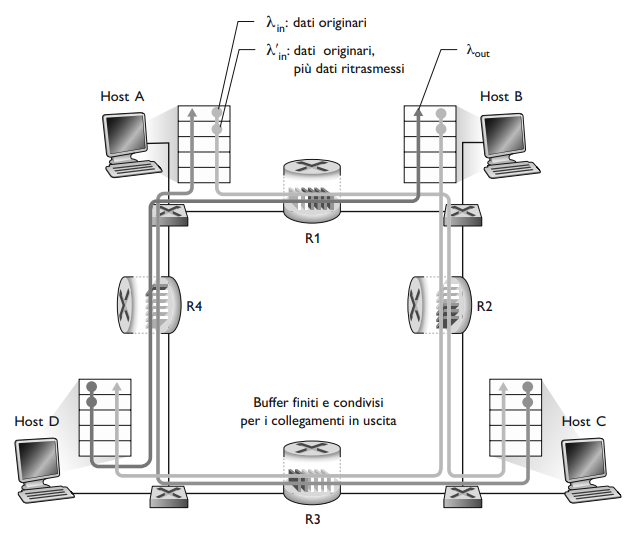
\includegraphics[width=0.5\textwidth]{img/scenario3.png}
\end{center}

\begin{itemize}
    \item \textbf{Basso Carico:} Per valori bassi di \(\lambda_{in}\), gli overflow dei buffer sono rari e il throughput (\(\lambda_{out}\)) è approssimativamente uguale al traffico inviato. Un aumento di \(\lambda_{in}\) porta a un aumento di \(\lambda_{out}\).
    \item \textbf{Alto Carico:} Per valori elevati di \(\lambda'_{in}\), il traffico da B a D compete con il traffico da A a C per le risorse del router R2. Il throughput di A-C diminuisce all'aumentare del traffico B-D, tendendo a 0 quando il traffico B-D tende all'infinito.
\end{itemize}

\begin{center}
  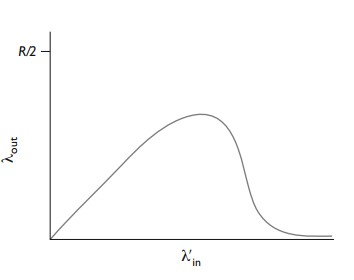
\includegraphics[width=0.4\textwidth]{img/scenario3diag.png}
\end{center}

\textbf{Costo della Congestione:}
\begin{itemize}
    \item Quando un pacchetto viene scartato, la capacità trasmissiva utilizzata sui collegamenti di upstream per instradare il pacchetto risulta sprecata.
\end{itemize}

\subsection{Controllo di congestione}
Bisogna limitare la trasmissione, si effettua mediante una "finestra di congestione" (\textbf{CongWin}), cioè una funzione dinamica della congestione.
\[\text{Frequenza d'invio} = \frac{\text{CongWin}}{\text{RTT}} \text{byte/sec}\]
Definiamola come una misura a spanne, non precisa.

Il mittente si accorge della congestione tramite il \textit{timeout} o il \textit{triplice ACK duplicato}.
Il mittente riduce la \textit{frequenza d'invio} dopo essersi accorto, con tre meccanismi:
\begin{enumerate}
  \item \textbf{Partenza lenta}: Stabilita la connessione si manda un solo pacchetto. All'inizio la velocità di trasmissione è molto lenta, poi crescerà a livello esponenziale finché non si verifica un evento di perdita, raddoppiamo la \textit{finestra di congestione} dopo ogni \textit{ACK ricevuto}. La \textit{partenza lenta} progredisce fino a un valore di soglia deciso dai progettisti.
    \begin{center}
    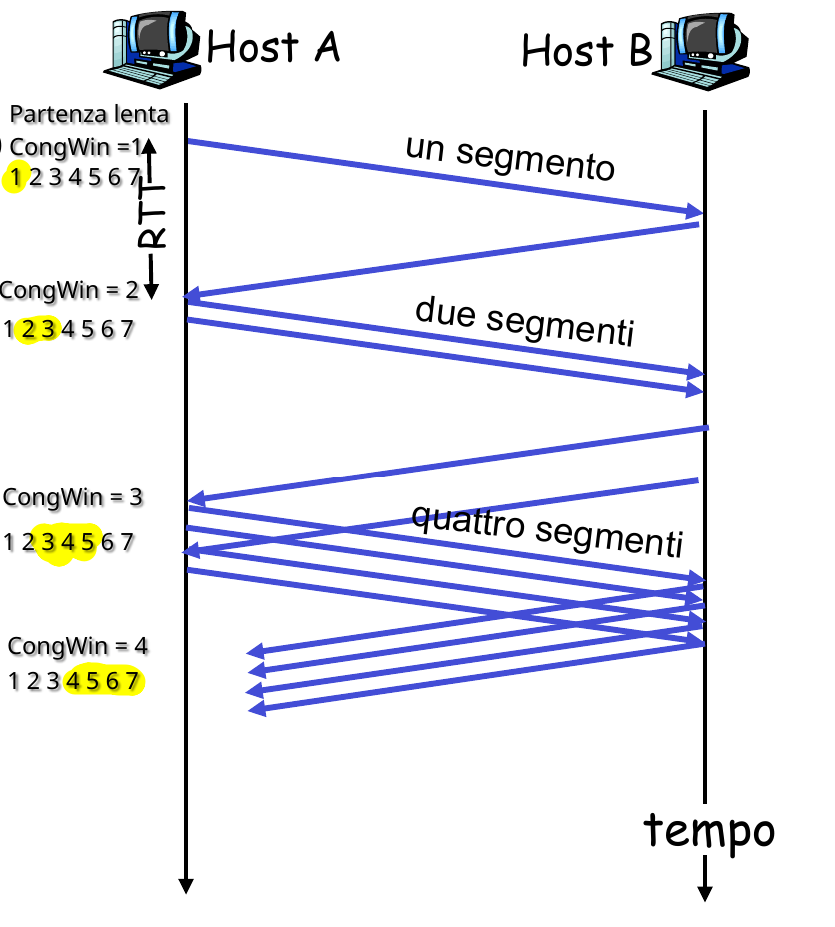
\includegraphics[width=\textwidth, height=7cm, keepaspectratio]{./img/partenzalenta.png}
    \end{center}
    Nel caso di \textit{triplice ACK duplicato} si passa all'algoritmo successivo per una crescita più lenta, impostando però:
    \[\text{valore di soglia} = \frac{\text{CongWin}}{2}\]
    \[\text{CongWin} = \text{valore di soglia}\]
  \item \textbf{AIMD}: Incremento additivo, decremento moltiplicativo in italiano. \textbf{Fase a regime}, dopo la partenza lenta. La crescita della \textit{finestra} continua in maniera lineare di \textbf{1 MSS} dopo ogni \textit{RTT}, nel caso di perdite la \textit{finestra} viene \textbf{dimezzata}. Questo è il suo andamento:
    \begin{center}
    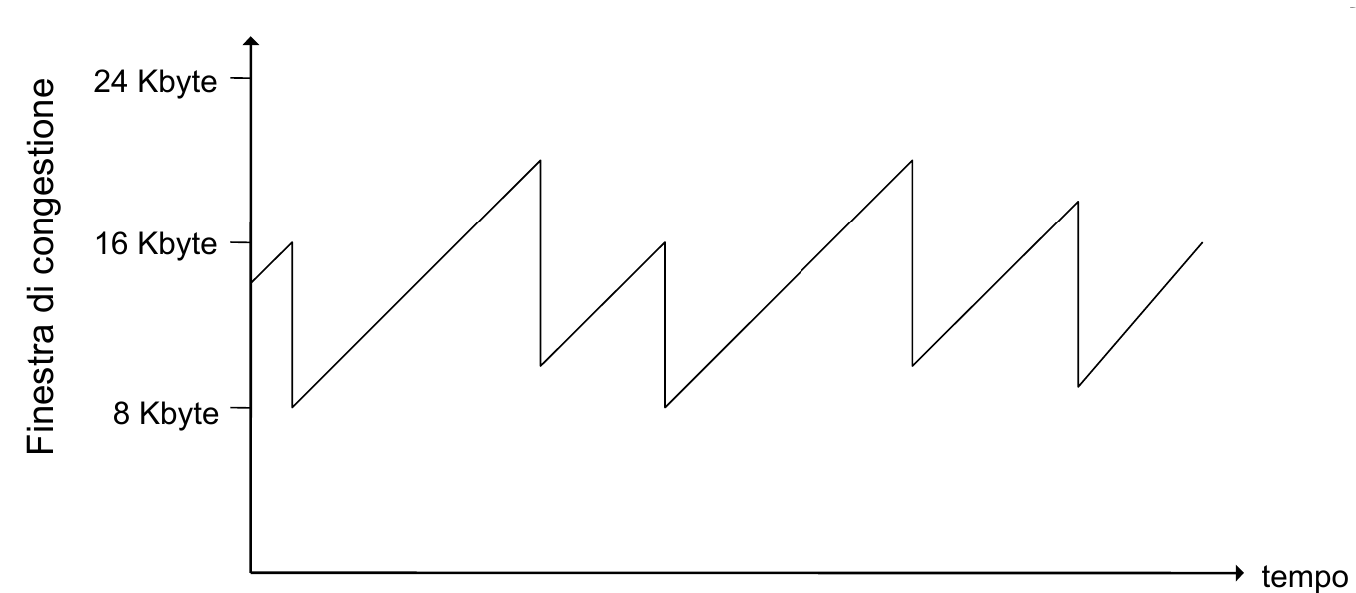
\includegraphics[width=\textwidth, height=4cm, keepaspectratio]{./img/AIMD.png}
    \end{center}
    Il suo funzionamento è così diagrammato:
    \begin{center}
    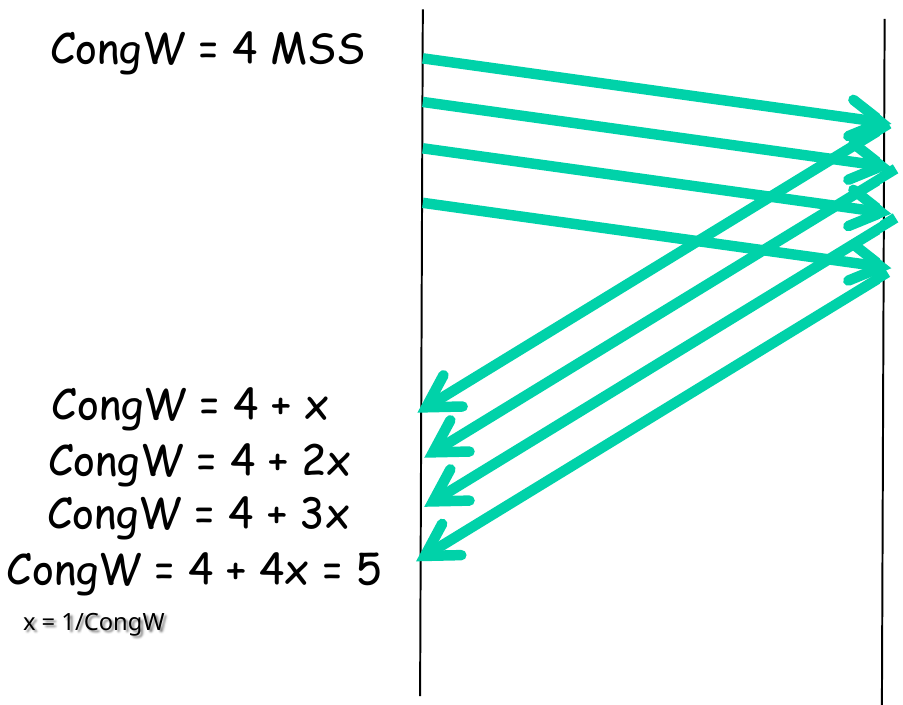
\includegraphics[width=\textwidth, height=5cm, keepaspectratio]{./img/AIMD-2.png}
    \end{center}
    negli esercizi, in caso di perdita di \textit{ACK}, arrotondiamo a +1 la frazione, solo per comodità. Nella realtà, essendo in byte, si fa il calcolo e si mantiene quel valore, non ci sono problemi in caso di perdita di ACK poiché l'ACK cumulativo conferma pure il pacchetto perso.
  \item \textbf{Reazione agli eventi di perdita}: Dividiamo i casi. Nel caso in cui si verifica il \textit{timeout} resettiamo la \textit{finestra} a 1, tornando così alla \textit{partenza lenta}, il valore di soglia viene impostato a
    \[\text{Valore di soglia} = \frac{\text{CongWin}}{2} \]
    \[\text{CongWin} = 1\]
    Nel caso in cui abbiamo una perdita (\textbf{Fast recovery}), \textit{triplice ACK duplicato}, imposto
    \[\text{CongWin} = \frac{\text{CongWin}}{2} \]
    \[\text{Valore di soglia} = \text{CongWin}\]
\end{enumerate}

\subsubsection*{Diagramma riassuntivo}
Il diagramma riassuntivo mostra i due stati principali del controllo di congestione TCP: \textit{slow start} e \textit{congestion avoidance}.

\begin{itemize}
    \item \textbf{Slow Start:} Inizia con una finestra di congestione (cwnd) di 1 MSS (Maximum Segment Size) e una soglia di slow start (ssthresh) di 64 KB. Il contatore di ACK duplicati (dupACKcount) è inizializzato a 0.
        \begin{itemize}
            \item \textit{Nuovo ACK:} Quando arriva un nuovo ACK, la finestra di congestione (cwnd) viene incrementata di 1 MSS, il contatore di ACK duplicati viene resettato a 0 e vengono inviati nuovi segmenti, se consentito.
            \item \textit{Timeout:} Se si verifica un timeout, la soglia di slow start (ssthresh) viene impostata a metà della finestra di congestione corrente, la finestra di congestione (cwnd) viene impostata a 1 MSS, il contatore di ACK duplicati viene resettato a 0 e viene ritrasmesso il segmento perso.
            \item \textit{Triplice ACK Duplicato:} Se si ricevono tre ACK duplicati, la soglia di slow start (ssthresh) viene impostata a metà della finestra di congestione corrente, la finestra di congestione (cwnd) viene impostata al valore della soglia e viene ritrasmesso il segmento perso.
        \end{itemize}
    \item \textbf{Congestion Avoidance:} Si entra in questo stato quando la finestra di congestione (cwnd) raggiunge o supera la soglia di slow start (ssthresh).
        \begin{itemize}
            \item \textit{Nuovo ACK:} Quando arriva un nuovo ACK, la finestra di congestione (cwnd) viene incrementata di 1 MSS * (MSS/cwnd), il contatore di ACK duplicati viene resettato a 0 e vengono inviati nuovi segmenti, se consentito.
            \item \textit{Timeout:} Se si verifica un timeout, la soglia di slow start (ssthresh) viene impostata a metà della finestra di congestione corrente, la finestra di congestione (cwnd) viene impostata a 1 MSS, il contatore di ACK duplicati viene resettato a 0 e viene ritrasmesso il segmento perso.
            \item \textit{Triplice ACK Duplicato:} Se si ricevono tre ACK duplicati, la soglia di slow start (ssthresh) viene impostata a metà della finestra di congestione corrente, la finestra di congestione (cwnd) viene impostata al valore della soglia e viene ritrasmesso il segmento perso.
        \end{itemize}
\end{itemize}

\begin{center}
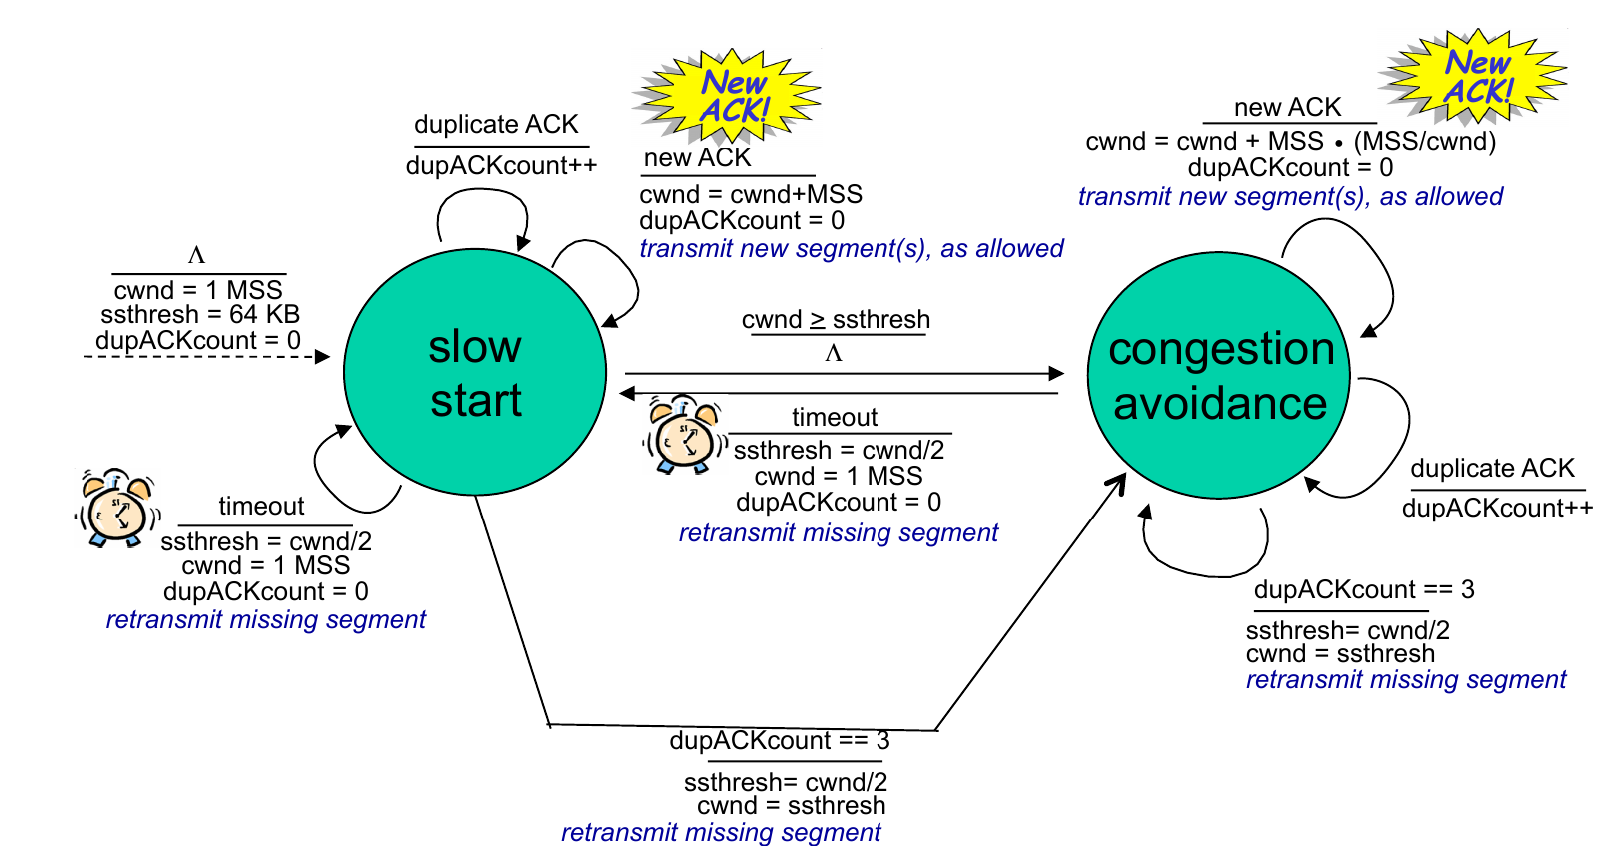
\includegraphics[width=\textwidth]{./img/diagrammacontrollodicongestione.png}
\end{center}

\subsection{Programmazione delle socket}

Le \textbf{socket} mettono in comunicazione \textit{livello applicativo} con il \textit{livello di trasporto}. Le socket sono \textit{endpoint} per la comunicazione. Esistono due tipi di \textit{socket}: \textbf{UDP} e \textbf{TCP}.

\subsubsection{Programmazione socket TCP}
Il \textit{server} crea una socket col comando \texttt{socket()}, inizialmente crea la \texttt{socket di benvenuto} per l'ascolto, quindi si crea una \textit{socket} senza parametri, bisogna comunicarglieli successivamente. Il server crea una \textit{socket di benvenuto} per l'ascolto e una \textit{socket di connessione} per ogni client.
Il \textit{server} aggancia i parametri alla \textit{socket} precedentemente creata tramite il comando \texttt{bind()}. Mettiamo il \textit{server} in stato di ascolto tramite il comando \texttt{listen()}.

Il \textit{client} crea una socket con i parametri del \textit{server}, tramite il comando \texttt{socket()}. Il \textit{client} aggancia i 4 parametri alla \textit{socket} precedentemente creata con il comando \texttt{bind()}. Il \textit{client} si connette al server mediante il comando \texttt{connect()}, la socket client è creata \textit{implicitamente} con il comando `connect()`. Il \textit{server} dall'altra parte accetterà la connessione sulla \textit{socket specifica} col comando \texttt{accept()}, e manda il messaggio \textbf{SYNACK}.
Il \textit{client} manda il messaggio al \textit{server} mediante il comando \texttt{send()} che verrà ricevuto dal comando \texttt{recv()} dal \textit{server}, mandando in risposta tramite \texttt{send()} l'\textbf{ACK}, che verrà ricevuto dal \textit{client} tramite \texttt{recv()}.

Si usa il comando \texttt{close()} per chiudere la connessione, possono mandarlo sia \textit{server} che \textit{client}, mandando il messaggio di \textbf{FIN}, ricevendo in risposta un \textbf{FINACK}.

\subsubsection*{\texttt{socket()}}
Creazione della \textit{socket}: \texttt{int s\_listen = socket(family, type, protocol);} \\
\texttt{family}: \texttt{AF\_INET} specifica IPV4 \\ \texttt{type}: \texttt{SOCK\_STREAM} per TCP, \texttt{SOCK\_DGRAM} per UDP \\ \texttt{protocol}: 0 (pseudo, IP). \\
Avremo un identificativo della socket come ritorno della funzione.

\subsubsection*{\texttt{bind()}}
Aggancio dei parametri alla \textit{socket} precedentemente creata vuota: \\
\texttt{bind(s\_listen = localAdd, AddLength);} \\
Si specifica la porta su cui mettersi in ascolto. `bind()` associa la socket a un \textit{indirizzo locale e una porta}. \\
s\_listen: identificatore della \textit{socket} \\
localAdd: di tipo \textbf{sockaddr\_in}, una struttura già definita. \\
AddLength: lunghezza della variabile localAdd \\
\begin{center}
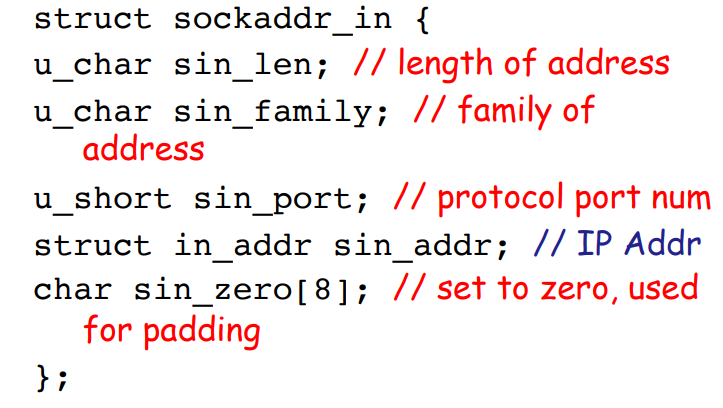
\includegraphics[width=\textwidth]{./img/struct_sockaddr_In.png}
\end{center}
L'immagine mostra la struttura \texttt{sockaddr\_in}, usata per specificare l'indirizzo e la porta a cui legare la socket.

Definisco \texttt{struct sockaddr\_in sockAdd;}
Imposto la famiglia: \texttt{sockAdd.sin\_family = AF\_INET;}
Per impostare l'indirizzo IPV4 abbiamo due modi:
\begin{enumerate}
  \item Specifichiamo l'indirizzo da ascoltare: \texttt{inet\_pton(AF\_INET, “127.0.0.1”, \&sockAdd.sin\_addr.s\_addr);}
  \item Ascolta da tutti gli indirizzi locali (in questo caso): \texttt{sockAdd.sin\_addr.s\_addr = htonl(INADDR\_ANY);}
\end{enumerate}
Imposto la porta: \texttt{sockAdd.sin\_port = htons(9999);}
\texttt{inet\_pton()} converte un indirizzo IP in formato testuale in un indirizzo IP in formato binario.
\texttt{htonl()} e \texttt{htons()} convertono un intero in un formato a 32 bit e 16 bit, rispettivamente, indipendente dall'architettura dell'host (big endian o little endian).

\subsubsection*{\texttt{listen()}}
\texttt{int status = listen(s\_listen, queuelength);} \\
Risultato: -1 errore, 0 ok \\
s\_listen: riferimento alla socket \\
queuelength: numero di client che possono stare in attesa. \\
È una funzione \textbf{non bloccante}, ritorna immediatamente un valore. `listen()` mette la socket in uno stato di \textit{ascolto passivo}.

\subsubsection*{\texttt{accept()}}
\texttt{int s\_new = accept(s\_listen, \&clientAddress, \&AddLength);} \\
s\_new: nuova socket per la comunicazione con il client, fino ad adesso abbiamo usato una \textit{socket di benvenuto}. \\
s\_listen: riferimento alla vecchia socket di benvenuto \\
clientAddress: riferimento alla struttura sockAddr\_in con l'indirizzo del client. \\
AddLength: dimensione della variabile clientAddress. \\
È una funzione \textbf{bloccante}, si \textit{blocca} fino a quando arriva una richiesta di connessione e quindi un \textbf{SYN}.

\subsubsection*{\texttt{send()}}
\texttt{int send(int s\_new, const void *buf, int len, int flags);} \\ 
s\_new: descrittore della socket \\
buf: puntatore al buffer \\
len: dimensione del buffer \\
flags: da impostare a 0. Questa funzione è usata per \textit{inviare dati} attraverso una socket.

\subsubsection*{\texttt{recv()}}
\texttt{int recv(int s\_new, void *buf, int len, unsigned int flags);} \\
Simile alla send. Questa funzione è usata per \textit{ricevere dati} attraverso una socket. \\
buf: conterrà i dati da ricevere.

\subsubsection*{\texttt{fork()}}
Funzione della libreria di C, \textbf{biforca} il \textit{processo}, creando \textbf{processo padre} e \textbf{processo figlio}, processi identici con stesse variabili. Il \textit{processo figlio} è una \textit{copia} del processo padre e gestirà le connessioni con il \textit{client} mentre col \textit{processo padre} gestiamo il \textit{listening}, rimanendo in \texttt{accept()}, ogni volta che gli arriverà una nuova richiesta per una socket faremo il \texttt{fork()} del processo padre, affidando al figlio la socket appena creata.

\subsubsection{Programmazione socket UDP}
Non esiste il comando \texttt{listen()} nella programmazione socket UDP, poiché non è un protocollo orientato alla connessione.

Per visualizzare i processi in corso, si può usare il comando \texttt{ps -ax}. Per visualizzare le socket aperte, si può usare il comando \texttt{netstat} (o \texttt{netstat -nap TCP} su macOS). Per terminare un processo, si può usare il comando \texttt{kill -9 <PID>}.
